\documentclass[
    table,
    12pt,
    oneside,
    a4paper,
    italian
]{book}

\setcounter{secnumdepth}{5}

% Definizione delle variabili direttamente nel documento principale
\newcommand{\myUni}{Università degli Studi di Padova}
\newcommand{\myDepartment}{Dipartimento di Matematica ``Tullio Levi-Civita''}
\newcommand{\myFaculty}{Corso di Laurea in Informatica}
\newcommand{\myTitle}{SviluppAbile: un'estensione per sviluppare pagine web accessibili con l'aiuto di un chatbot}
\newcommand{\myDegree}{Tesi di Laurea Triennale}
\newcommand{\profTitle}{Prof.ssa}
\newcommand{\myProf}{Ombretta Gaggi}
\newcommand{\graduateTitle}{Laureanda}
\newcommand{\myName}{Elena Chilese}
\newcommand{\myStudentID}{2008074}
\newcommand{\myAA}{2024-2025}
\newcommand{\myLocation}{Padova}
\newcommand{\myTime}{Settembre 2025}

% Caricamento dei pacchetti
% Pacchetti di base  
\usepackage{colorprofiles}
\usepackage[a-1a,mathxmp]{pdfx}[2018/12/22] % crea PDF/A-1a

% Set di caratteri, lingua, grafica
\usepackage[T1]{fontenc}
\usepackage{lmodern}
\usepackage[utf8]{inputenc}
\usepackage[italian]{babel}
\usepackage[dvipsnames]{xcolor} 
\usepackage{graphicx}
\usepackage{caption}
\usepackage{subcaption}

% Layout di pagina
\usepackage[
  top=2.75cm,
  bottom=2.75cm,
  right=2.75cm,
  left=2.75cm,
  includehead,
  includefoot
]{geometry}
\usepackage{fancyhdr}
\usepackage{setspace}
\usepackage{emptypage}
\usepackage{indentfirst}

% Sezioni, titoli, citazioni
\usepackage{titlesec}
\usepackage{sectsty}
\usepackage{quoting}[font=small]
\usepackage{csquotes}

\usepackage{array}
\newcolumntype{C}[1]{>{\centering\arraybackslash}p{#1}}
\usepackage{longtable}
\usepackage{etoolbox}

% -- centra automaticamente *ogni* longtable --
\makeatletter
\pretocmd\LT@start{%
  \setlength{\LTleft}{\fill}%
  \setlength{\LTright}{\fill}%
}{}{}
\makeatother

\usepackage{tabularx}
\usepackage{tabulary}
\usepackage{adjustbox}
\usepackage{hhline}

% Landscape (reset centraggio dentro landscape)
\usepackage{pdflscape}
\AtBeginEnvironment{landscape}{%
  \setlength{\LTleft}{0pt}%
  \setlength{\LTright}{0pt}%
}

% Float & utilità
\usepackage{placeins}   % \FloatBarrier
\usepackage{tikz}


% Struttura documento, riferimenti interni
\usepackage{bookmark}
\usepackage{nameref}
\usepackage[italian]{varioref}
\usepackage{zref-totpages}

% extra
\usepackage{comment}
\usepackage{epigraph}
\usepackage{lipsum}
\usepackage{listings}
\usepackage{float}
%\usepackage{minted}

% Biblio + glossario
\usepackage[backend=biber, backref, style=numeric]{biblatex}
\usepackage[toc, acronym]{glossaries}

% Altro
\usepackage{mparhack,relsize}
\usepackage{chngpage, calc}
\usepackage[bottom]{footmisc}
\usepackage{pifont}

% Hyperref 
\usepackage{hyperref}

\PassOptionsToPackage{dvipsnames}{xcolor} % colori PDF/A

\usepackage{colorprofiles}
% PDF/A
% validate in https://www.pdf-online.com/osa/validate.aspx

% Caricamento della configurazione della tesi
% Define custom colors
\definecolor{hyperColor}{HTML}{0B3EE3}
\definecolor{tableGray}{HTML}{F5F5F7}
\definecolor{veryPeri}{HTML}{6667ab}

\definecolor{lightgray}{rgb}{.9,.9,.9}
\definecolor{darkgray}{rgb}{.4,.4,.4}
\definecolor{purple}{rgb}{0.65, 0.12, 0.82}
\definecolor{editorGray}{rgb}{1.0, 1.0, 1.0}
\definecolor{editorOcher}{rgb}{1, 0.5, 0} % #FF7F00 -> rgb(239, 169, 0)
\definecolor{editorGreen}{rgb}{0, 0.5, 0} % #007C00 -> rgb(0, 124, 0)

% Set chapter font size
\chapterfont{\fontsize{24}{22}\selectfont}

% Set line height
\linespread{1.5}

% Custom hyphenation rules
\hyphenation{
    data-base
    al-go-rithms
    soft-ware
}

\begin{filecontents*}{\jobname.xmpdata}
  \Title{SviluppAbile: un'estensione per sviluppare pagine web accessibili con l'aiuto di un chatbot}
  \Author{Elena Chilese} 
  \Language{it-IT}
  \Subject{Realizzazione di un'estensione web con integrazione di un chatbot IA per l'analizzare ed aiutare a creare pagine web accessibili}
  \Keywords{Accessibilità \sep Chatbot}
\end{filecontents*} 

% Images path
\graphicspath{{img/}}

% Force page color
\pagecolor{white}

% Better spacing for footnotes
\setlength{\skip\footins}{5mm}
\setlength{\footnotesep}{5mm}

% Fix header height warning
\setlength{\headheight}{27.11652pt}
\addtolength{\topmargin}{-12.61652pt}

% Add glossary subscript
\newcommand{\glox}{\textsubscript{\textbf{\textit{G}}}}

% Paragraph formatting
\titleformat{\paragraph}
{\normalfont\normalsize\bfseries}{\theparagraph}{1em}{}
\titlespacing*{\paragraph}
{0pt}{3.25ex plus 1ex minus .2ex}{1.5ex plus .2ex}

% Keep chapter format with "Chapter X" but modify spacing
\titleformat{\chapter}[display]
    {\normalfont\huge\bfseries}
    {\chaptertitlename\ \thechapter}
    {10pt}   % Reduced space between "Chapter X" and the title
    {\Huge}

% Reduce spacing before and after the chapter
\titlespacing*{\chapter}
    {0pt}    % left margin
    {-50pt}   % space before title (reduced from default 50pt)
    {20pt}   % space after title (reduced from default 40pt)

\newcommand{\chapterintroline}[1]{%
    \begin{quote}
    \normalfont
    #1
    \end{quote}
    \centerline{\rule{0.5\textwidth}{0.5pt}}  % Adds a horizontal line
}

% Page styling
\pagestyle{fancy}
\fancyhf{}
\fancyhead[L]{\leftmark}
\fancyfoot[C]{\thepage}

% Utility commands
\newcommand\blankpage{
\clearpage
    \begingroup
    \null
    \thispagestyle{empty}
    \hypersetup{pageanchor=false}
    \clearpage
\endgroup
}

\newcommand\blankpagewithnumber{
  \clearpage
  \thispagestyle{plain}
  \null
  \clearpage
}

\newcommand\increasepagenumbering{
    \addtocounter{page}{+1}
}

% Load glossaries
% Acronyms

\newacronym{css}{CSS}{Cascading Style Sheets}
\newacronym{dom}{DOM}{Document Object Model}
\newacronym{js}{JS}{JavaScript}
\newacronym{html}{HTML}{HyperText Markup Language}

\newacronym{ui}{UI}{User Interface}
\newacronym{aria}{ARIA}{Accessible Rich Internet Applications}
\newacronym{wcag}{WCAG}{Web Content Accessibility Guidelines}
\newacronym{mcag}{MCAG}{Mobile Content Accessibility Guidelines}
\newacronym[description={\glslink{apig}{\textit{Application Program Interface}}}]
    {api}{API}{\textit{Application Program Interface}}
\newacronym{loc}{LOC}{Lines of Code}

\newacronym[description={\glslink{iag}{\textit{Artificial Intelligence}}}]
    {ai}{AI}{\textit{Artificial Intelligence}}

\newacronym[description={\glslink{iag}{Intelligenza Artificiale}}]
    {ia}{IA}{Intelligenza Artificiale}
\newacronym[description={\glslink{llmg}{\textit{Large Language Model}}}]
    {llm}{LLM}{\textit{Large Language Model}}
\newacronym[description={\glslink{w3cg}{\textit{World Wide Web Consortium}}}]
    {w3c}{W3C}{\textit{World Wide Web Consortium}}
\newacronym[description={\glslink{xmlg}{\textit{Extensible Markup Language}}}]
    {xml}{XML}{\textit{Extensible Markup Language}}
\newacronym[description={\glslink{urlg}{\textit{Uniform Resource Locator}}}]
    {url}{URL}{\textit{Uniform Resource Locator}}
\newacronym[description={\glslink{gpug}{\textit{Graphics Processing Unit}}}]
    {gpu}{GPU}{\textit{Graphics Processing Unit}}
\newacronym{mv2}{MV2}{Manifest V2}
\newacronym{mv3}{MV3}{Manifest V3}
\newacronym{poc}{PoC}{\glslink{pocg}{\textit{Proof of Concept}}}
\newacronym{tcp}{TCP}{\glslink{tcpg}{\textit{Transmission Control Protocol}}}
\newacronym{tv}{TV}{Total Validator}

% Glossary

\newglossaryentry{apig} {
    name=\acrshort{api},
    text=Application Program Interface,
    sort=api,
    description={in informatica con il termine \emph{Application Programming Interface} (ing. interfaccia di programmazione di un'applicazione) si indicano regole e specifiche per la comunicazione tra \textit{software}. \\
    Tali regole fungono da interfaccia tra i vari \textit{software} e ne facilitano l’interazione, allo stesso modo in cui l’interfaccia utente facilita l’interazione tra uomo e \textit{computer}. \\
    \cite{site:api-treccani}
    }
}

\newglossaryentry{aig} {
    name=\acrshort{ia},
    text=Artificial Intelligence,
    sort=ai,
    description={insieme di studi e tecniche, pertinenti all’informatica, ma prossime alle ricerche di logica matematica e con profonde implicazioni sia filosofiche sia sociali, che mirano alla realizzazione di macchine o programmi in grado di risolvere problemi e di riprodurre attività proprie dell’intelligenza umana o che comunque ne simulino il comportamento. \\
    \cite{site:ai-treccani}
    }
}

\newglossaryentry{domg}{ 
    name={\acrshort{dom}},
    text={Document Object Model},
    sort=dom,
    description={in informatica il Document Object Model (spesso abbreviato come \acrshort{dom}), lett. "modello a oggetti del documento", è una forma di rappresentazione dei documenti strutturati come modello orientato agli oggetti. È lo standard ufficiale del \acrshort{w3c} per la rappresentazione di documenti strutturati in maniera da essere neutrali sia per la lingua che per la piattaforma. \\
    \cite{site: dom-wiki}}
}

\newglossaryentry{backendg}{
    name=\textit{Backend},
    text=\textit{Backend},
    sort=back-end,
    description= {con il termine \textit{"backend"} si intende la parte non visibile all'utente di un programma, che elabora e gestisce i dati generati dall'interfaccia grafica.\\
    \cite{site:backend-wiki}
    }
}

\newglossaryentry{llmg}{
    name=\acrshort{llm},
    text={Large Language Model},
    sort=llm,
    description= {con il termine \textit{"Large Language Model"} si intende un algoritmo di \glslink{iag}{intelligenza artificiale} che, processando massivamente una grande quantità di dati, utilizza tecniche di \textit{deep learning} in vari ambiti dell’elaborazione del linguaggio naturale come la comprensione, la traduzione, la generazione e la previsione di nuovi contenuti.\\
    \cite{site:llm-treccani}
    }
}


\newglossaryentry{w3cg}{
    name=\acrshort{w3c},
    text={W3C},
    sort=w3c,
    description= {il \textit{World Wide Web Consortium}, anche conosciuto come \acrshort{w3c}, è un'organizzazione non governativa internazionale che ha come scopo quello di favorire lo sviluppo di tutte le potenzialità del \glslink{wwwg}{World Wide Web} e diffondere la cultura dell'accessibilità della Rete.\\
    \cite{site:w3c-wiki}
    }
}

\newglossaryentry{wwwg}{
    name=\textit{World Wide Web},
    text={World Wide Web},
    sort=world-wide-web,
    description= {il \textit{World Wide Web} (termine in lingua inglese traducibile in italiano come "rete di ampiezza mondiale" o "rete mondiale"), è uno dei principali servizi di Internet, che permette di navigare e usufruire di un insieme molto vasto di contenuti, multimediali e non, interrelati tramite collegamenti ipertestuali (\textit{link}), e di fruire di ulteriori servizi accessibili a tutti o ad una parte selezionata degli utenti di Internet (mediante autenticazione).\\
    \cite{site:www-wiki}
    }
}

\newglossaryentry{xmlg}{
    name=\textit{eXtensible Markup Language},
    text={eXtensible Markup Language},
    sort=extensible-markup-language,
    description= {in informatica, l'\acrshort{xml} (sigla di \textit{eXtensible Markup Language}, lett. "linguaggio di marcatura estendibile") è un metalinguaggio per la definizione di linguaggi di \glslink{markupg}{markup}, ovvero un linguaggio basato su un meccanismo sintattico che consente di definire e controllare il significato degli elementi contenuti in un documento o in un testo.\\
    \cite{site:xml-wiki}
    }
}

\newglossaryentry{urlg}{
    name=\acrshort{url},
    text={Uniform Resource Locator},
    sort=url,
    description= {nel linguaggio informatico, sigla dell’ingl.\textit{Uniform Resource Locator} «localizzatore unico della risorsa (informatica)», indirizzo di un sito web espresso in modo univoco e con una forma utilizzabile dal \glslink{browserg}{browser}.\\
    \cite{site:url-treccani}
    }
}

\newglossaryentry{gpug}{
    name=\acrshort{gpu},
    text={Graphics Processing Unit},
    sort=gpu,
    description= {l'unità di elaborazione grafica (in acronimo \acrshort{gpu}, dall'inglese \textit{Graphics Processing Unit}), è un processore progettato per accelerare la creazione di immagini in un frame buffer, destinato all'output su un dispositivo di visualizzazione. \\
     \cite{site:gpu-wiki}
    }
}

\newglossaryentry{chatbotg}{
    name=\textit{Chatbot},
    text={Chatbot},
    sort=chatbot,
    description= {è un software progettato per simulare una conversazione con un essere umano. \\
     \cite{site:chatbot-wiki}
    }
}

\newglossaryentry{pluging}{
    name=\textit{Plugin},
    text={Plugin},
    sort=plugin,
    description= {in campo informatico è un programma non autonomo che interagisce con un altro programma per ampliarne o estenderne le funzionalità originarie. \\
     \cite{site:plugin-wiki}
    }
}

\newglossaryentry{markupg}{
    name=\textit{Markup},
    text={Markup},
    sort=markup,
    description= {un linguaggio di \textit{markup} (in italiano linguaggio di marcatura o linguaggio di formattazione) è un insieme di regole che descrivono i meccanismi di rappresentazione (strutturali, semantici, presentazionali) o d'impaginazione di un testo. \\
     \cite{site:markup-wiki}
    }
}

\newglossaryentry{formg}{
    name=\textit{Form},
    text={Form},
    sort=form,
    description= {in Internet, modulo telematico a disposizione dell’utente per l’inserimento e l’invio di dati. \\
     \cite{site:form-treccani}
    }
}

\newglossaryentry{browserg}{
    name=\textit{Browser},
    text={Browser},
    sort=browser,
    description= {nel linguaggio informatico, programma di un computer che permette il collegamento alla rete Internet e mediante il quale si può navigare da un sito telematico all’altro. \\
     \cite{site:browser-treccani}
    }
}

\newglossaryentry{scriptg}{
    name=\textit{Script},
    text={Script},
    sort=script,
    description= {in informatica, programma o sequenza di istruzioni che viene interpretata o portata a termine da un altro programma. \\
     \cite{site:script-treccani}
    }
}

\newglossaryentry{asincronog}{
    name=Asincrono,
    text={Asincrono},
    sort=asincrono,
    description= {non sincrono, che non avviene o si manifesta cioè nel medesimo tempo, o, in senso più tecnico, che manca di sincronismo. \\
     \cite{site:asincrono-treccani}
    }
}

\newglossaryentry{client-sideg}{
    name=\textit{Client-side},
    text={Client-side},
    sort=client-side,
    description= {in informatica, nell'ambito delle reti di calcolatori, il termine lato client (client-side in inglese) indica le operazioni di elaborazione effettuate da un client in un'architettura client-server. \\
     \cite{site:client_side-wiki}
    }
}

\newglossaryentry{serverg}{
    name=\textit{Server},
    text={Server},
    sort=server,
    description= {in informatica (con riferimento a una rete di calcolatori), calcolatore che svolge funzioni di servizio per tutti i calcolatori collegati. \\
     \cite{site:server-treccani}
    }
}

\newglossaryentry{cloud-computingg}{
    name=\textit{Cloud computing},
    text={Cloud computing},
    sort=cloud-computing,
    description= {la tecnologia che, sotto forma di servizio offerto dal provider al cliente, permette di memorizzare e di elaborare i dati e i programmi di un utente grazie all’utilizzo di risorse hardware o software distribuite in rete. \\
     \cite{site:cloud_computing-treccani}
    }
}

\newglossaryentry{latenzag}{
    name=Latenza,
    text={Latenza},
    sort=latenza,
    description= {in informatica, il tempo impiegato da un’informazione per andare da un’unità all’altra di un sistema, in partic. da un sensore al relativo elaboratore (è detto anche l. di risposta). \\
     \cite{site:latenza-treccani}
    }
}

\newglossaryentry{quantizzazioneg}{
    name=Quantizzazione,
    text={Quantizzazione},
    sort=quantizzazione,
    description= {in elettronica e nella tecnica delle telecomunicazioni, l’operazione, attuata con un quantizzatore, consistente nel suddividere il campo di variabilità di una grandezza continua in un numero finito di intervalli (definiti a volte «quanti»), in ciascuno dei quali la grandezza è considerata costante e sostituita con un valore rappresentativo. \\
     \cite{site:quantizzazione-treccani}
    }
}

\newglossaryentry{open-sourceg}{
    name=\textit{Open source},
    text={Open source},
    sort=open-source,
    description= {in informatica, software non protetto da copyright, il cui codice sorgente è lasciato alla disponibilità degli utenti e quindi liberamente modificabile. \\
     \cite{site:open_source-treccani}
    }
}

\newglossaryentry{debuggingg}{
    name=\textit{Debugging},
    text={Debugging},
    sort=debugging,
    description= {nel linguaggio dell’informatica, operazione di messa a punto di un programma, un’applicazione, ecc., consistente nella ricerca (di norma effettuata dall’elaboratore) e nella correzione (talvolta automatica) degli errori di procedura, relativi al tipo di linguaggio impiegato, che impediscono o rendono difettosa l’elaborazione. \\
     \cite{site:debugging-treccani}
    }
}

\newglossaryentry{desktop-firstg}{
    name=\textit{Desktop-first},
    text={Desktop-first},
    sort=desktop-first,
    description= { significa progettare il sito web avendo come obiettivo principale l'esperienza su desktop. Sebbene sarebbe facile pensare che il desktop-first sia un approccio ormai superato, in realtà esistono diverse ragioni per cui molti scelgono ancora di partire in grande e poi ridimensionare. \\
     \cite{site:desktop_first-hvdig}
    }
}

\newglossaryentry{iag}{
    name=\textit{Intelligenza Artificiale},
    text={Intelligenza artificiale},
    sort=intelligenza-artificiale,
    description= { insieme di studi e tecniche, pertinenti all’informatica, ma prossime alle ricerche di logica matematica e con profonde implicazioni sia filosofiche sia sociali, che mirano alla realizzazione di macchine o programmi in grado di risolvere problemi e di riprodurre attività proprie dell’intelligenza umana o che comunque ne simulino il comportamento. \\
     \cite{site:ai-treccani}
    }
}

\newglossaryentry{ChatGPTg} {
    name=\textit{ChatGPT},
    text=ChatGPT,
    sort=ChatGPT,
    description={ implementazione del modello di intelligenza artificiale (\acrshort{ia}) sviluppato da OpenAI, basato sull'architettura GPT-3 (Generative Pre-trained Transformer 3) e progettato per comprendere e generare testo in linguaggio naturale. \\
    \cite{site:chatgpt-treccani}
    }
}

\newglossaryentry{Chrome-basedg} {
    name=\textit{Chrome-based},
    text=Chrome-based,
    sort=Chrome-based,
    description={ un \glslink{browserg}{browser} o software che utilizza la base del codice sorgente del progetto \glslink{open-sourceg}{open-source} Chromium, la stessa foundation di Google Chrome.
    }
}

\newglossaryentry{gitg} {
    name=\textit{GIT},
    text=GIT,
    sort=GIT,
    description={ è un'applicazione software per il controllo di versione distribuito utilizzabile da interfaccia a riga di comando, creato da Linus Torvalds nel 2005. \\
    \cite{site:git-wiki}
    }
}

\newglossaryentry{pocg} {
    name=\acrshort{poc},
    text=Proof of Concept,
    sort=poc,
    description={ è una realizzazione incompleta o abbozzata (sinopsi) di un determinato progetto o metodo per dimostrare la fattibilità o confermare la validità di alcuni principi o concetti fondamentali. Un esempio tipico è quello di un prototipo. \\
    \cite{site:poc-wiki}
    }
}

\newglossaryentry{webassemblyg} {
    name=\textit{WebAssembly},
    text=WebAssembly,
    sort=webAssembly,
    description={ è uno standard web che definisce un formato binario e un corrispondente formato testuale per la scrittura di codice eseguibile nelle pagine web. Ha lo scopo di abilitare l'esecuzione del codice quasi alla stessa velocità con cui esegue il codice macchina nativo. \\
    \cite{site:webassembly-wiki}
    }
}

\newglossaryentry{websocketg} {
    name=\textit{WebSocket},
    text=WebSocket,
    sort=websocket,
    description={ è un protocollo che fornisce canali di comunicazione full-duplex (trasmissione bidirezionale simultanea) attraverso una singola connessione \acrshort{tcp}. \\
    \cite{site:websocket-wiki}
    }
}

\newglossaryentry{tcpg} {
    name=\acrshort{tcp},
    text=Transmission Control Protocol,
    sort=transmission-control-protocol,
    description={ è un protocollo di rete a pacchetto di livello di trasporto, appartenente alla suite di protocolli Internet, che si occupa di controllo della trasmissione ovvero rendere affidabile la comunicazione dati in rete tra mittente e destinatario. \\
    \cite{site:tcp-wiki}
    }
}

\newglossaryentry{open-weightg} {
    name=\textit{Open weight},
    text=Open weight,
    sort=open-weight,
    description={ i modelli a peso aperto sono sistemi di \glslink{iag}{intelligenza artificiale} in cui i “pesi” effettivi, i numeri fondamentali che il modello ha appreso durante l’addestramento, sono resi pubblici. Questi pesi sono ciò che guida le previsioni, le risposte e il comportamento generale del modello. \\
    \cite{site:open_weight-invezz}
    }
}
\glsaddallunused
\makeglossaries
\renewcommand*{\glstextformat}[1]{\textit{#1}\glox}

% Bibliography setup
\addbibresource{references/bibliography.bib}
\defbibheading{bibliography}{
    \cleardoublepage
    \phantomsection
    \addcontentsline{toc}{chapter}{\bibname}
    \chapter*{\bibname\markboth{\bibname}{\bibname}}
}

% Add this to suppress split bibliography warning
\BiblatexSplitbibDefernumbersWarningOff

% Hyperref setup
\hypersetup{
    colorlinks=true,
    linktocpage=true,
    pdfstartpage=1,
    pdfstartview=,
    breaklinks=true,
    pdfpagemode=UseNone,
    pageanchor=true,
    pdfpagemode=UseOutlines,
    plainpages=false,
    bookmarksnumbered,
    bookmarksopen=true,
    bookmarksopenlevel=1,
    hypertexnames=true,
    pdfhighlight=/O,
    allcolors = hyperColor
}

% Caption setup
\captionsetup{
    tableposition=top,
    figureposition=bottom,
    font=small,
    format=hang,
    labelfont=bf
}

% Adjust the way tables are handled
\setlength{\tabcolsep}{4pt}  % Default is 6pt, reducing gives more space in tables

% For longtable format
\setlength\LTleft{0pt}
\setlength\LTright{0pt}

% Adjust the way floats are handled to avoid excessive whitespace
\renewcommand{\topfraction}{0.9}        % Default 0.7
\renewcommand{\bottomfraction}{0.9}     % Default 0.3
\renewcommand{\textfraction}{0.1}       % Default 0.2
\renewcommand{\floatpagefraction}{0.85} % Default 0.5
\setcounter{topnumber}{3}              % Default 2
\setcounter{bottomnumber}{3}           % Default 1
\setcounter{totalnumber}{5}            % Default 3

% Enhanced color definitions for code
\definecolor{codeBackground}{HTML}{F8F9FA}
\definecolor{codeBorder}{HTML}{DEE2E6}
\definecolor{jsKeyword}{HTML}{D73A49}        % Red for keywords
\definecolor{jsString}{HTML}{0A3B78}         % Dark blue for strings
\definecolor{jsComment}{HTML}{6A737D}        % Gray for comments
\definecolor{jsNumber}{HTML}{005CC5}         % Blue for numbers
\definecolor{jsFunction}{HTML}{008052}       % Emerald for functions
\definecolor{jsVariable}{HTML}{E36209}       % Orange for variables
\definecolor{jsOperator}{HTML}{D73A49}       % Red for operators
\definecolor{lineNumbers}{HTML}{6A737D}      % Gray for line numbers

% Enhanced JavaScript language definition
\lstdefinelanguage{JavaScript}{
  keywords={
    % Control flow
    if, else, switch, case, default, break, continue, return,
    % Loops
    for, while, do, 
    % Functions and classes
    function, async, await, class, constructor, extends, super,
    % Variables
    var, let, const,
    % Types and values
    true, false, null, undefined, typeof, instanceof,
    % Error handling
    try, catch, finally, throw,
    % Others
    new, this, delete, in, of, with, debugger, export, import, from, as
  },
  keywordstyle=\color{jsKeyword}\bfseries,
  % Secondary keywords (built-in objects and methods)
  ndkeywords={
    % Built-in objects
    Array, Object, String, Number, Boolean, Date, RegExp, Math, JSON,
    console, window, document, setTimeout, setInterval, clearTimeout, clearInterval,
    Promise, Error, TypeError, ReferenceError,
    % Common methods
    log, push, pop, shift, unshift, slice, splice, map, filter, reduce, forEach,
    getElementById, querySelector, addEventListener, fetch, then, catch
  },
  ndkeywordstyle=\color{jsFunction}\bfseries,
  % Strings
  stringstyle=\color{jsString},
  morestring=[b]",
  morestring=[b]',
  morestring=[b]`,
  % Comments
  comment=[l]{//},
  morecomment=[s]{/*}{*/},
  commentstyle=\color{jsComment}\itshape,
  % Numbers
  sensitive=true,
  % Additional styling
  identifierstyle=\color{black},
  % Operators
  otherkeywords={
    =, +, -, *, /, \%, ==, ===, !=, !==, <, >, <=, >=, &&, ||, !, 
    +=, -=, *=, /=, ++, --, =>, ?, :, ;, \{, \}, [, ], (, )
  },
  % Special handling for template literals
  moredelim=[s][\color{jsString}]{`}{`}
}

% Enhanced HTML5 language definition (keeping your existing one but with better colors)
\lstdefinelanguage{HTML5}{
    language=html,
            sensitive=true, 
            alsoletter={<>=-},
            otherkeywords={
            % HTML tags
            <, </, >,
            </a, <a, </a>,
            </abbr, <abbr, </abbr>,
            </address, <address, </address>,
            </area, <area, </area>,
            </area, <area, </area>,
            </article, <article, </article>,
            </aside, <aside, </aside>,
            </audio, <audio, </audio>,
            </audio, <audio, </audio>,
            </b, <b, </b>,
            </base, <base, </base>,
            </bdi, <bdi, </bdi>,
            </bdo, <bdo, </bdo>,
            </blockquote, <blockquote, </blockquote>,
            </body, <body, </body>,
            </br, <br, </br>,
            </button, <button, </button>,
            </canvas, <canvas, </canvas>,
            </caption, <caption, </caption>,
            </cite, <cite, </cite>,
            </code, <code, </code>,
            </col, <col, </col>,
            </colgroup, <colgroup, </colgroup>,
            </data, <data, </data>,
            </datalist, <datalist, </datalist>,
            </dd, <dd, </dd>,
            </del, <del, </del>,
            </details, <details, </details>,
            </dfn, <dfn, </dfn>,
            </div, <div, </div>,
            </dl, <dl, </dl>,
            </dt, <dt, </dt>,
            </em, <em, </em>,
            </embed, <embed, </embed>,
            </fieldset, <fieldset, </fieldset>,
            </figcaption, <figcaption, </figcaption>,
            </figure, <figure, </figure>,
            </footer, <footer, </footer>,
            </form, <form, </form>,
            </h1, <h1, </h1>,
            </h2, <h2, </h2>,
            </h3, <h3, </h3>,
            </h4, <h4, </h4>,
            </h5, <h5, </h5>,
            </h6, <h6, </h6>,
            </head, <head, </head>,
            </header, <header, </header>,
            </hr, <hr, </hr>,
            </html, <html, </html>,
            </i, <i, </i>,
            </iframe, <iframe, </iframe>,
            </img, <img, </img>,
            </input, <input, </input>,
            </ins, <ins, </ins>,
            </kbd, <kbd, </kbd>,
            </keygen, <keygen, </keygen>,
            </label, <label, </label>,
            </legend, <legend, </legend>,
            </li, <li, </li>,
            </link, <link, </link>,
            </main, <main, </main>,
            </map, <map, </map>,
            </mark, <mark, </mark>,
            </math, <math, </math>,
            </menu, <menu, </menu>,
            </menuitem, <menuitem, </menuitem>,
            </meta, <meta, </meta>,
            </meter, <meter, </meter>,
            </nav, <nav, </nav>,
            </noscript, <noscript, </noscript>,
            </object, <object, </object>,
            </ol, <ol, </ol>,
            </optgroup, <optgroup, </optgroup>,
            </option, <option, </option>,
            </output, <output, </output>,
            </p, <p, </p>,
            </param, <param, </param>,
            </pre, <pre, </pre>,
            </progress, <progress, </progress>,
            </q, <q, </q>,
            </rp, <rp, </rp>,
            </rt, <rt, </rt>,
            </ruby, <ruby, </ruby>,
            </s, <s, </s>,
            </samp, <samp, </samp>,
            </script, <script, </script>,
            </section, <section, </section>,
            </select, <select, </select>,
            </small, <small, </small>,
            </source, <source, </source>,
            </span, <span, </span>,
            </strong, <strong, </strong>,
            </style, <style, </style>,
            </summary, <summary, </summary>,
            </sup, <sup, </sup>,
            </svg, <svg, </svg>,
            </table, <table, </table>,
            </tbody, <tbody, </tbody>,
            </td, <td, </td>,
            </template, <template, </template>,
            </textarea, <textarea, </textarea>,
            </tfoot, <tfoot, </tfoot>,
            </th, <th, </th>,
            </thead, <thead, </thead>,
            </time, <time, </time>,
            </title, <title, </title>,
            </tr, <tr, </tr>,
            </track, <track, </track>,
            </u, <u, </u>,
            </ul, <ul, </ul>,
            </var, <var, </var>,
            </video, <video, </video>,
            </wbr, <wbr, </wbr>,
            />, <!
  },  
  ndkeywords={
    % General
            =,
            % HTML attributes
            accept=, accept-charset=, accesskey=, action=, align=, alt=, async=, autocomplete=, autofocus=, autoplay=, autosave=, bgcolor=, border=, buffered=, challenge=, charset=, checked=, cite=, class=, code=, codebase=, color=, cols=, colspan=, content=, contenteditable=, contextmenu=, controls=, coords=, data=, datetime=, default=, defer=, dir=, dirname=, disabled=, download=, draggable=, dropzone=, enctype=, for=, form=, formaction=, headers=, height=, hidden=, high=, href=, hreflang=, http-equiv=, icon=, id=, ismap=, itemprop=, keytype=, kind=, label=, lang=, language=, list=, loop=, low=, manifest=, max=, maxlength=, media=, method=, min=, multiple=, name=, novalidate=, open=, optimum=, pattern=, ping=, placeholder=, poster=, preload=, pubdate=, radiogroup=, readonly=, rel=, required=, reversed=, rows=, rowspan=, sandbox=, scope=, scoped=, seamless=, selected=, shape=, size=, sizes=, span=, spellcheck=, src=, srcdoc=, srclang=, start=, step=, style=, summary=, tabindex=, target=, title=, type=, usemap=, value=, width=, wrap=,
            % CSS properties
            accelerator:,azimuth:,background:,background-attachment:,
            background-color:,background-image:,background-position:,
            background-position-x:,background-position-y:,background-repeat:,
            behavior:,border:,border-bottom:,border-bottom-color:,
            border-bottom-style:,border-bottom-width:,border-collapse:,
            border-color:,border-left:,border-left-color:,border-left-style:,
            border-left-width:,border-right:,border-right-color:,
            border-right-style:,border-right-width:,border-spacing:,
            border-style:,border-top:,border-top-color:,border-top-style:,
            border-top-width:,border-width:,bottom:,caption-side:,clear:,
            clip:,color:,content:,counter-increment:,counter-reset:,cue:,
            cue-after:,cue-before:,cursor:,direction:,display:,elevation:,
            empty-cells:,filter:,float:,font:,font-family:,font-size:,
            font-size-adjust:,font-stretch:,font-style:,font-variant:,
            font-weight:,height:,ime-mode:,include-source:,
            layer-background-color:,layer-background-image:,layout-flow:,
            layout-grid:,layout-grid-char:,layout-grid-char-spacing:,
            layout-grid-line:,layout-grid-mode:,layout-grid-type:,left:,
            letter-spacing:,line-break:,line-height:,list-style:,
            list-style-image:,list-style-position:,list-style-type:,margin:,
            margin-bottom:,margin-left:,margin-right:,margin-top:,
            marker-offset:,marks:,max-height:,max-width:,min-height:,
            min-width:,transition-duration:,transition-property:,
            transition-timing-function:,transform:,
            -moz-transform:,-moz-binding:,-moz-border-radius:,
            -moz-border-radius-topleft:,-moz-border-radius-topright:,
            -moz-border-radius-bottomright:,-moz-border-radius-bottomleft:,
            -moz-border-top-colors:,-moz-border-right-colors:,
            -moz-border-bottom-colors:,-moz-border-left-colors:,-moz-opacity:,
            -moz-outline:,-moz-outline-color:,-moz-outline-style:,
            -moz-outline-width:,-moz-user-focus:,-moz-user-input:,
            -moz-user-modify:,-moz-user-select:,orphans:,outline:,
            outline-color:,outline-style:,outline-width:,overflow:,
            overflow-X:,overflow-Y:,padding:,padding-bottom:,padding-left:,
            padding-right:,padding-top:,page:,page-break-after:,
            page-break-before:,page-break-inside:,pause:,pause-after:,
            pause-before:,pitch:,pitch-range:,play-during:,position:,quotes:,
            -replace:,richness:,right:,ruby-align:,ruby-overhang:,
            ruby-position:,-set-link-source:,size:,speak:,speak-header:,
            speak-numeral:,speak-punctuation:,speech-rate:,stress:,
            scrollbar-arrow-color:,scrollbar-base-color:,
            scrollbar-dark-shadow-color:,scrollbar-face-color:,
            scrollbar-highlight-color:,scrollbar-shadow-color:,
            scrollbar-3d-light-color:,scrollbar-track-color:,table-layout:,
            text-align:,text-align-last:,text-decoration:,text-indent:,
            text-justify:,text-overflow:,text-shadow:,text-transform:,
            text-autospace:,text-kashida-space:,text-underline-position:,top:,
            unicode-bidi:,-use-link-source:,vertical-align:,visibility:,
            voice-family:,volume:,white-space:,widows:,width:,word-break:,
            word-spacing:,word-wrap:,writing-mode:,z-index:,zoom:
  },
  keywordstyle=\color{jsKeyword}\bfseries,
  ndkeywordstyle=\color{jsFunction},
  morecomment=[s]{<!--}{-->},
  commentstyle=\color{jsComment}\itshape,
  stringstyle=\color{jsString},
  tag=[s]
}

% Enhanced global lstset configuration
\lstset{
  % Basic styling
  basicstyle=\ttfamily\footnotesize,
  backgroundcolor=\color{codeBackground},
  % Frame and spacing
  frame=single,
  framerule=0.5pt,
  rulecolor=\color{codeBorder},
  framesep=4pt,
  framexleftmargin=6pt,
  framextopmargin=4pt,
  framexbottommargin=4pt,
  % Line numbers
  numbers=left,
  numberstyle=\tiny\color{lineNumbers},
  numbersep=12pt,
  stepnumber=1,
  % Text formatting
  showstringspaces=false,
  showspaces=false,
  showtabs=false,
  tabsize=2,
  % Line breaking
  breaklines=true,
  breakatwhitespace=true,
  prebreak=\raisebox{0ex}[0ex][0ex]{\ensuremath{\hookleftarrow}},
  postbreak=\raisebox{0ex}[0ex][0ex]{\ensuremath{\hookrightarrow\space}},
  % Margins and positioning
  xleftmargin=20pt,
  xrightmargin=5pt,
  % Caption positioning
  captionpos=b,
  % Language settings
  language=JavaScript,
  alsolanguage=HTML5,
  % Extended character support
  extendedchars=true,
  inputencoding=utf8,
  % Special character handling
  literate=%
    {à}{{\'a}}1 {è}{{\'e}}1 {ì}{{\'i}}1 {ò}{{\'o}}1 {ù}{{\'u}}1
    {À}{{\'A}}1 {È}{{\'E}}1 {Ì}{{\'I}}1 {Ò}{{\'O}}1 {Ù}{{\'U}}1
    {ä}{{\"{a}}}1 {ö}{{\"{o}}}1 {ü}{{\"{u}}}1
    {Ä}{{\"{A}}}1 {Ö}{{\"{O}}}1 {Ü}{{\"{U}}}1 {ß}{{\ss}}1
    {€}{{\euro}}1
}

% Specialized settings for different code types
\lstdefinestyle{jsStyle}{
  language=JavaScript,
  keywordstyle=\color{jsKeyword}\bfseries,
  stringstyle=\color{jsString},
  commentstyle=\color{jsComment}\itshape,
  numberstyle=\tiny\color{lineNumbers},
  identifierstyle=\color{black},
  emphstyle=\color{jsFunction}\bfseries
}

\lstdefinestyle{htmlStyle}{
  language=HTML5,
  keywordstyle=\color{jsKeyword}\bfseries,
  ndkeywordstyle=\color{jsFunction},
  stringstyle=\color{jsString},
  commentstyle=\color{jsComment}\itshape,
  numberstyle=\tiny\color{lineNumbers}
}

\date{}
\hypersetup{pdfstartview=}

\begin{document}
    \frontmatter
    \begin{titlepage}
    \begin{center}
        \begin{Large}
            \textbf{\myUni}\\
        \end{Large}

        \vspace{5pt}

        \begin{large}
            \textsc{\myDepartment}\\
        \end{large}

        \vspace{5pt}

        \begin{large}
            \textsc{\myFaculty}\\
        \end{large}

        \vspace{25pt}
        
        \begin{figure}[htbp]
            \centering
            
\includegraphics[alt={Emblema dell'Università degli Studi di Padova}, height=6cm]{img/logo_unipd.png}
        \end{figure}

        \begin{Large}
            \textbf{\myTitle}\\
        \end{Large}

        \vspace{5pt}

        \begin{large}
            \textit{\myDegree}\\
        \end{large}

        \vspace{50pt}
        
        \begin{normalsize}
            \begin{flushleft}
                \textit{Relatrice}\\
                \profTitle\ \myProf
            \end{flushleft}

            \vspace{-48pt}
            
            \begin{flushright}
                \textit{\graduateTitle}\\
                \myName\\
                \textit{Matricola} \myStudentID
            \end{flushright}
        \end{normalsize}

        \vspace*{\fill}
        
        \line(1, 0){338} \\
        \begin{normalsize}
            \textsc{Anno Accademico \myAA}
        \end{normalsize}
    \end{center}
\end{titlepage}
    \clearpage
\phantomsection
\thispagestyle{empty}
\hfill
\vfill

{\small\noindent\textcopyright\ \myName, \myTime. Tutti i diritti riservati. \myDegree: ``\textit{\myTitle}'', \myUni, \myDepartment.}
    \increasepagenumbering
    \cleardoublepage
\phantomsection
\pdfbookmark{Acknowledgements}{Acknowledgements}

\begin{flushright}{
    \slshape
    ``Dedicata ad Elena, che mai si è arresa...''} \\
\end{flushright}

\begingroup
\let\clearpage\relax
\let\cleardoublepage\relax

\chapter*{Ringraziamenti}
\noindent\begin{small}Per prima cosa desidero ringraziare la professoressa Ombretta Gaggi, relatrice della mia tesi e tutor del mio stage, per l’assistenza e il sostegno fornitimi durante tutto il percorso di stage e nella stesura del lavoro.\\
Un sincero grazie va anche a Salvatore Gatto per il supporto e l’aiuto durante lo stage.\\

\noindent Con profondo affetto ringrazio i miei genitori e, in particolar modo, mia mamma, per la pazienza e la forza con cui mi ha sempre sostenuta anche nei momenti più difficili. Un ringraziamento va anche ai miei zii e soprattutto a mio nonno Adriano, per la vicinanza e l’affetto che non mi ha mai fatto mancare.\\

\noindent Un grazie speciale a Michele, che mi è stato accanto fin dall’inizio del percorso universitario, diventando non solo un prezioso punto di riferimento in ogni occasione, ma anche il mio compagno di avventure e il mio migliore amico.

\noindent Ringrazio di cuore tutti i miei amici e i compagni di università (in particolare Matteo, Elena ed Erica) per la loro vicinanza e il sostegno dimostrato in questi anni.\\

\noindent Desidero esprimere la mia gratitudine inoltre ai colleghi e ai professori dell’ITE Fusinieri, che hanno contribuito al mio percorso con il loro supporto e i loro insegnamenti.\\
\end{small}
\vspace{0.75cm}

\noindent{\myLocation, \myTime}
\hfill \textit{\myName}

\endgroup
    
    \cleardoublepage
\phantomsection
\pdfbookmark{Sommario}{Sommario}
\begingroup
\let\clearpage\relax
\let\cleardoublepage\relax
\chapter*{Sommario}

\noindent Il presente documento descrive il lavoro svolto durante il periodo di stage, della durata di trecento ore svolto presso il Dipartimento di Matematica “Tullio Levi-Civita” dell’Università di Padova. \\
Il prodotto finale dello stage è un'estensione web \glslink{Chrome-basedg}{Chrome-based\glox} per aiutare gli sviluppatori web nella creazione di pagine web accessibili.\\
\\
Gli obiettivi del progetto sono:
\begin{itemize}
    \item Studio dell'accessibilità web;
    \item Studio di Manifest V3;
    \item Studio delle possibili \glslink{api}{\acrshort{api}\glox} per l'integrazione dell' \glslink{ia}{\acrshort{ia}\glox};
    \item Creazione di un'estensione web che integri un \glslink{chatbotg}{chatbot\glox} \glslink{ai}{\acrshort{ai}\glox} per analizzare il codice sorgente della pagina web ed offrire risposte adeguate.
\end{itemize}

\endgroup
\vfill
    \cleardoublepage
\renewcommand{\contentsname}{Tabella dei contenuti}
\pdfbookmark{\contentsname}{tableofcontents}
\setcounter{secnumdepth}{5}
\setcounter{tocdepth}{5}     
\tableofcontents
\clearpage
\begingroup
    \let\clearpage\relax
    \let\cleardoublepage\relax
    \let\cleardoublepage\relax
    % Figures list
    \phantomsection
    \renewcommand{\listfigurename}{Elenco delle figure}
    \pdfbookmark{\listfigurename}{edf}
    \listoffigures
    \vspace*{8ex}
    % Tables list
    \phantomsection
    \renewcommand{\listtablename}{Elenco delle tabelle}
    \pdfbookmark{\listtablename}{edt}
    \listoftables
    % Listings list
\endgroup
\cleardoublepage
    
    \mainmatter
    \definecolor{darkblue}{RGB}{0,0,139}

\hypersetup{
  colorlinks=true,
  linkcolor=blue,   % sezioni, figure, tabelle in blu
  citecolor=blue,   % bibliografia
  urlcolor=darkblue  % link esterni
}

\chapter{Introduzione}
\label{chap:intro}

\noindent L’accessibilità web rappresenta un aspetto fondamentale per garantire che tutte le persone, indipendentemente dalle loro abilità o disabilità, possano utilizzare i contenuti digitali in modo efficace. Le linee guida \glslink{wcag}{\acrshort{wcag}\glox} (\textit{Web Content Accessibility Guidelines}) sono uno standard internazionale, esse definiscono i criteri tecnici per migliorare l’accessibilità dei siti web, intervenendo su aspetti quali la struttura semantica, la navigazione tramite tastiera, il contrasto cromatico dei colori e la compatibilità con tecnologie assistive.\\ 
Un sito accessibile non solo migliora l’esperienza d’uso per persone con disabilità visive, motorie o cognitive, ma estende anche la fruibilità a un pubblico più ampio, contribuendo a un web più inclusivo e universale.\\ 
Nonostante ciò, spesso la realizzazione pratica di siti accessibili incontra difficoltà dovute a scarsa conoscenza delle best-practices dello sviluppo web accessibile, delle normative in questione e della scarsa diffusione di strumenti automatizzati efficaci.


\section{L'idea del progetto}
\noindent Il progetto sviluppato durante il mio stage si inserisce all’interno di un’iniziativa molto più ampia intitolata \textit{“Supporting Accessibility Auditing and HTML Validator using Large Language Models”} a cui partecipano e collaborano docenti e stagisti dell’Università di Padova e dell’Università di Bologna.\\
Tale progetto nasce dall’esigenza di affrontare il problema dell’accessibilità web, diritto fondamentale per tutti i cittadini (in particolare per le persone con disabilità) che devono poter accedere alle informazioni sul web senza barriere.\\
Nonostante le normative nazionali e internazionali (come la \textit{Direttiva Europea sull'Accessibilità Web} e l' \textit{European Accessibility Act}) impongano requisiti chiari, una buona parte dei siti web presenta ancora numerose criticità di accessibilità. \cite{site:UE_accessibility_act}\\
In questo contesto, il progetto mira a valutare, testare e sfruttare le capacità dei \textit{Large Language Models} (\glslink{llm}{\acrshort{llm}\glox}) per supportare l’audit dell’accessibilità e la validazione del codice \glslink{html}{\acrshort{html}\glox}.\\
L’obiettivo finale è sviluppare strumenti innovativi che utilizzino modelli di \glslink{iag}{intelligenza artificiale\glox}, come \glslink{ChatGPTg}{ChatGPT\glox}, per fornire un supporto interattivo agli sviluppatori, aiutandoli a identificare e correggere problematiche di accessibilità in modo più efficace e comprensibile rispetto ai metodi tradizionali. Attraverso questa integrazione, si intende migliorare la qualità e soprattutto la chiarezza dei risultati e favorire una cultura più diffusa sull’accessibilità digitale.\\ Inoltre, si vuole anche valutare se gli LLM siano effettivamente in grado di svolgere questo tipo di lavoro.\\
\\
L’estensione \textit{“SviluppAbile”} è un primo esempio di strumento per lo sviluppo guidato di pagine web accessibili.
Essa nasce dall’esigenza di supportare gli sviluppatori web nel creare pagine accessibili in modo semplice e interattivo, sfruttando le potenzialità dell’\glslink{iag}{intelligenza artificiale}.\\
L’estensione \glslink{Chrome-basedg}{Chrome-based} sviluppata offre due modalità principali: \begin{itemize}
    \item una modalità di analisi assistita, che permette di ispezionare il \glslink{dom}{\acrshort{dom}\glox} di una pagina web e di porre domande specifiche sull’accessibilità, ottenendo risposte chiare e contestualizzate; 
    \item una modalità di sviluppo guidato, in cui l’utente riceve suggerimenti di codice accessibile in tempo reale, visualizzati in una colonna centrale e pronti per essere copiati o scaricati.
\end{itemize}
Questo duplice approccio consente di integrare nel flusso di lavoro quotidiano degli sviluppatori un valido supporto basato sull'\acrshort{ia}, con l’obiettivo di facilitare il rispetto delle linee guida \acrshort{wcag} e migliorare la qualità complessiva del codice.

\section{Analisi delle soluzioni già presenti}
\noindent Sul mercato esistono diversi strumenti e \glslink{pluging}{plugin\glox} dedicati alla verifica dell’accessibilità delle pagine web, come Total Validator (vedi paragrafo \ref{subsec:tv}), WAVE (vedi paragrafo \ref{subsec:wave}) e Lighthouse (vedi paragrafo \ref{subsec:lighthouse}), che offrono principalmente funzionalità di scansione automatica e generazione di report.\\ 
Questi strumenti, tuttavia, forniscono spesso una panoramica statica dei problemi riscontrati; indicano chiaramente dove si trova l’errore, ma i risultati sono generalmente formulati in modo formale e destinati ad un esperto di accessibilità. Di conseguenza, l’utente non specialista deve interpretare autonomamente le informazioni, con il rischio di applicare soluzioni non sempre pienamente conformi alle linee guida.\\ 
Alcuni software integrano suggerimenti o tutorial, ma raramente utilizzano modelli di \glslink{iag}{intelligenza artificiale} in grado di interagire con lo sviluppatore in linguaggio naturale, rispondendo a domande specifiche o guidandolo direttamente nella scrittura del codice. \\
\\
\textit{“SviluppAbile”} si distingue per l’integrazione di una chat \acrshort{ia} che funge da assistente personale, e per la duplice modalità operativa che combina l’analisi in tempo reale con un supporto diretto allo sviluppo, colmando così una lacuna importante nelle soluzioni attualmente disponibili.

\section{Organizzazione del testo}
\noindent Il documento è diviso in sei capitoli e illustra in maniera dettagliata l’esperienza di stage svolta.

\begin{description}
    \item Il {\hyperref[chap:analisi-requisiti]{secondo capitolo}} illustra le informazioni raccolte in fase di analisi del progetto tramite requisiti e casi d’uso.
    \item Il {\hyperref[chap:linguaggi-tecnologie]{terzo capitolo}} approfondisce le tecnologie e gli strumenti utilizzati per la realizzazione del progetto.
    \item Il {\hyperref[chap:sviluppo]{quarto capitolo}} descrive lo sviluppo dell’estensione, evidenziando le scelte progettuali e le soluzioni implementative.
    \item Il {\hyperref[chap:test]{ quinto capitolo}} presenta i test effettuati, volti a valutare l’effettiva utilità dell’estensione rispetto agli strumenti tradizionali di validazione del codice accessibile.
    \item Il {\hyperref[chap:conclusioni]{ sesto capitolo}} riassume i risultati ottenuti e le possibili evoluzioni future del progetto. 
\end{description}

\noindent Riguardo la stesura del testo, relativamente al documento sono state adottate le seguenti convenzioni tipografiche:
\begin{itemize}
	\item Gli acronimi, le abbreviazioni e i termini ambigui o di uso non comune menzionati vengono definiti nel glossario, situato alla fine del presente documento;
	\item Per i termini riportati nel glossario viene utilizzata la seguente nomenclatura: \glslink{apig}{Application Programming Interface\glox};
	\item I termini in lingua straniera o facenti parti del gergo tecnico sono evidenziati con il carattere \textit{corsivo};
	\item Gli esempi di codice, le domande poste all'IA e le righe di codice utilizzano il formato \texttt{monospace}.
\end{itemize}

\newpage

% COSE UTILI
%Lorem Figure \ref{fig:entanglement}
%Esempio di utilizzo di un termine nel glossario \gls{api}.
%Esempio di citazione direttamente nel testo \cite{site:agile-manifesto}.
%Esempio di citazione nel piè di pagina \footcite{womak:lean-thinking}.
    \chapter{Analisi dei requisiti}
\label{chap:analisi-requisiti}
%\footnote{\cite{site:agile-manifesto}} per citare

\section{Obiettivo del progetto}
\label{sec:obiettivo}
\noindent L’obiettivo principale del progetto è la realizzazione di un’estensione web interattiva con chatbot integrato, pensata per supportare gli sviluppatori nell’individuazione e nella correzione degli errori di accessibilità presenti nelle pagine web. \\Il progetto si propone di rispondere alle seguenti esigenze:
\begin{itemize}
    \item Fornire un linguaggio chiaro e facilmente comprensibile, anche per chi non ha conoscenze approfondite delle linee guida di accessibilità;
    \item Offrire un supporto immediato e contestuale durante lo sviluppo del codice;
    \item Facilitare il miglioramento della qualità e dell’accessibilità dei siti web, promuovendo buone pratiche di progettazione inclusiva.
\end{itemize}

\section{Casi d'uso}
\label{sec:uc}

\section{Tracciamento dei requisiti}
\label{sec:rq}
    \chapter{Tecnologie}
\label{chap:linguaggi-tecnologie}
%\footnote{\cite{site:agile-manifesto}} per citare

\section{Linguaggi}
\subsection{HTML}
\label{subsec:html}
\noindent \acrshort{html} (\textit{HyperText Markup Language}) è il linguaggio di marcatura standard utilizzato per strutturare i contenuti delle pagine web. Non si tratta di un linguaggio di programmazione, ma di uno strumento che consente di definire gli elementi presenti su una pagina (come titoli, testi, immagini, link, \glslink{formg}{form}) assegnando loro un significato semantico tramite l’uso di tag. \\
Introdotto nel 1991 da Tim Berners-Lee, \acrshort{html} si è evoluto nel tempo attraverso diverse versioni, fino a diventare uno standard globale supervisionato dal \textit{World Wide Web Consortium} (\acrshort{w3c}).\\
\\
La struttura di un file \acrshort{html} si basa su una serie di elementi, rappresentati attraverso tag, che permettono di definire la natura e la funzione dei contenuti all'interno di una pagina web. Ogni tag descrive una tipologia specifica di contenuto o un comportamento associato, contribuendo all'organizzazione semantica del documento. I tag sono delimitati da parentesi angolari (\texttt{< >}) e, nella maggior parte dei casi, sono utilizzati in coppie: un tag di apertura e uno di chiusura, quest’ultimo contraddistinto da una barra (\texttt{</tag>}). Alcuni elementi, tuttavia, non necessitano di chiusura e sono detti auto-chiudenti, come ad esempio \texttt{<img>} per l’inserimento di immagini, o \texttt{<br>} per i ritorni a capo. Questa struttura gerarchica e nidificata consente al \glslink{browserg}{browser} di interpretare correttamente i contenuti, garantendo coerenza tra presentazione e significato.\\
\\
La versione attuale, HTML5 (logo in figura \ref{fig:logo_HTML5}), è stata rilasciata in modo stabile nel 2014.\\
HTML5 rappresenta un’evoluzione del linguaggio di \glslink{markupg}{markup} con l’obiettivo di ridurre la dipendenza da \glslink{pluging}{plugin} esterni, introducendo nuove funzionalità native. Tra le principali novità vi sono gli elementi \texttt{<canvas>}, \texttt{<video>} e \texttt{<audio>}, nuovi tag semantici per strutturare i contenuti (come articoli, intestazioni, sezioni) e controlli avanzati per i \glslink{formg}{form} (email, \acrshort{url}, numeri, date, ricerca). 
\\Vengono inoltre introdotti strumenti per la memorizzazione locale dei dati sul client tramite \texttt{localStorage} e \texttt{sessionStorage}.

\begin{figure}[H]
    \centering
    
\includegraphics[width=0.25\textwidth, alt={Logo HTML5}]{img/html5.png}
    \caption[Logo HTML5]{Logo HTML5}\label{fig:logo_HTML5}
\end{figure}

\subsection{CSS}
\label{subsec:css}
\noindent \acrshort{css} (\textit{Cascading Style Sheets}) è un linguaggio utilizzato per definire la presentazione dei documenti \acrshort{html} e \acrshort{xml}. Introdotto nel 1996 da Håkon Wium Lie, consente di separare la struttura dei contenuti dalla loro formattazione, migliorando la chiarezza del codice e facilitandone la manutenzione.\\ 
I fogli di stile permettono di specificare, tramite regole composte da selettori, proprietà e valori, l’aspetto degli elementi \acrshort{html}: layout, colori, font, margini, spaziature, effetti visivi, animazioni e molto altro. Le regole di stile possono essere inline (tramite tag \texttt{<style>} o con attributi style) oppure riportate in file esterni .css riutilizzabili. La prima soluzione non mantiene però una netta separazione tra struttura e contenuto, non rispettando quindi le best-practice del settore.\\ 
L'attuale versione, CSS3 (logo in figura \ref{fig:logo_CSS3}), è modulare e introduce importanti funzionalità come \texttt{flexbox}, \texttt{grid}, media query per il responsive design, transizioni, trasformazioni e nuovi selettori.
\begin{figure}[H]
    \centering
    
\includegraphics[width=0.25\textwidth, alt={Logo CSS3}]{img/css3.png}
    \caption[Logo CSS3]{Logo CSS3}\label{fig:logo_CSS3}
\end{figure}

\subsection{Prism.js}
\label{subsec:prism}
\noindent Prism.js è una libreria JavaScript leggera ed estensibile progettata per evidenziare la sintassi del codice sorgente in modo chiaro e leggibile, rispettando gli standard moderni del web. \\
Supporta un’ampia gamma di linguaggi di programmazione e di \glslink{markupg}{markup}, ed è facilmente personalizzabile tramite temi e \glslink{pluging}{plugin}. \\
Grazie alla sua efficienza e semplicità di integrazione, viene utilizzata in milioni di siti web per migliorare la leggibilità del codice, rendendolo più comprensibile sia a sviluppatori che a utenti. E’ disponibile in diverse varianti, sia per il white-mode che per il dark-mode.\\
Nella mia estensione, Prism.js è stato integrato per colorare il codice sorgente del \acrshort{dom}, facilitando l’analisi e la comprensione della struttura \acrshort{html}.

\subsection{JavaScript}
\label{subsec:js}
\noindent JavaScript (logo in figura \ref{fig:logo_JS}) è un linguaggio di programmazione dinamico, interpretato ed orientato agli oggetti, progettato originariamente per rendere le pagine web interattive.\\ 
È stato sviluppato nel 1995 da Brendan Eich per Netscape con il nome LiveScript, e successivamente rinominato in JavaScript per motivi di marketing, pur non avendo legami diretti con il linguaggio Java. La sua standardizzazione è gestita da \textit{ECMA International}, sotto il nome ECMAScript.\\
\\
Concepito per essere eseguito direttamente all’interno del \glslink{browserg}{browser}, JavaScript consente di scrivere \glslink{scriptg}{script} incorporati nel codice \acrshort{html}, eseguibili senza compilazione al momento del caricamento della pagina. Questi \glslink{scriptg}{script} permettono di manipolare il \acrshort{dom} (Document Object Model), reagire agli eventi dell’utente (come click, input da tastiera o movimenti del mouse), modificare dinamicamente il contenuto della pagina e gestire funzionalità come validazioni, messaggi, animazioni, e interazioni \glslink{asincronog}{asincrone}.\\
Oltre alla manipolazione di elementi visivi, JavaScript permette di sfruttare numerose \acrshort{api} messe a disposizione dal \glslink{browserg}{browser}, dalla gestione del mouse e del touch, alla manipolazione delle immagini, fino alla gestione locale dei dati attraverso meccanismi come il LocalStorage. Questa versatilità lo rende uno strumento fondamentale per lo sviluppo di applicazioni web moderne.\\
\\
JavaScript si è evoluto da semplice linguaggio \glslink{client-sideg}{client-side} a tecnologia completa e versatile, oggi utilizzabile anche su \glslink{serverg}{server} (ad esempio con \textit{Node.js}) e in ambienti esterni ai \glslink{browserg}{browser} grazie all’uso di diversi motori JavaScript i quali permettono l’esecuzione di codice \acrshort{js} con alte prestazioni, rendendo il linguaggio adatto anche a contesti \glslink{backendg}{backend}, applicazioni desktop e mobile.\\
Oggi JavaScript rappresenta uno dei tre pilastri fondamentali del web, insieme a \acrshort{html} e \acrshort{css}, ed è completamente integrato con essi. Esistono anche linguaggi alternativi (come TypeScript o CoffeeScript) che vengono compilati in JavaScript, offrendo funzionalità aggiuntive mantenendo la compatibilità con l’ambiente JavaScript standard.
\begin{figure}[H]
    \centering
    
\includegraphics[width=0.2\textwidth, alt={Logo JS}]{img/javascript.png}
    \caption[Logo JavaScript]{Logo JavaScript}\label{fig:logo_JS}
\end{figure}

\section{Tecnologie e strumenti}
\subsection{Chrome Extension}
\label{subsec:chromeExt}
\noindent Le estensioni di Chrome sono piccoli programmi software che consentono di arricchire e personalizzare il \glslink{browserg}{browser}, aggiungendo funzionalità aggiuntive o migliorando quelle già esistenti.\\
Grazie ad esse è possibile modificare l’interfaccia utente, automatizzare attività ripetitive, integrare servizi esterni e rendere più efficiente la navigazione sul web.\\ 
La distribuzione delle estensioni avviene principalmente tramite il \textit{Chrome Web Store}, ma durante le fasi di sviluppo è possibile installarle manualmente utilizzando la modalità sviluppatore disponibile nel \glslink{browserg}{browser}.

\subsubsection{Manifest V3}
\label{subsec:mv3}
\noindent Manifest V3 (\acrshort{mv3}) è la specifica più recente per la creazione di estensioni per Chrome e altri \glslink{browserg}{browser} basati su \textit{Chromium}. \\Rispetto alla precedente Manifest V2, l'ultima versione introduce diverse modifiche per migliorare la sicurezza, le prestazioni e la privacy delle estensioni. \cite{site:mv3-chrome} \\
Questa nuova versione è una risposta alle criticità emerse con il Manifest V2, e introduce cambiamenti strutturali significativi nel modo in cui le estensioni interagiscono con il \glslink{browserg}{browser} e le pagine web.\\
E' importante notare che Manifest V3 non è retrocompatibile con le estensioni V2 senza modifiche sostanziali e che la versione è tuttora in evoluzione, poiché alcune funzionalità sono ancora in fase di implementazione.\\
Il file \texttt{manifest.json} in \acrshort{mv3} continua a rappresentare il cuore dell’estensione, definendo metadati fondamentali come nome, versione, permessi richiesti e \glslink{scriptg}{script} da eseguire. Tuttavia, rispetto a \acrshort{mv2}, \acrshort{mv3} impone restrizioni più rigide su quali \acrshort{api} possono essere utilizzate e introduce un modello di esecuzione più efficiente e sicuro.\\

\noindent Gli elementi principali di un’estensione basata su Manifest V3 sono:
\begin{itemize}
    \item \textbf{Manifest}: come nelle versioni precedenti, il file \texttt{manifest.json} contiene tutte le informazioni necessarie per il funzionamento dell’estensione, inclusi i permessi richiesti. 
    Tra i permessi più rilevanti vi sono: \begin{itemize}
        \item downloads: permette all’estensione di avviare e gestire download di file, ad esempio per salvare contenuti generati o analizzati;
        \item scripting: consente l’esecuzione di \glslink{scriptg}{script} personalizzati nelle pagine web, utile per analizzare o modificare il \acrshort{dom};
        \item activeTab: garantisce l’accesso temporaneo alla scheda attiva dopo un interazione dell’utente con l’estensione;
        \item tabs: fornisce informazioni sulle schede del \glslink{browserg}{browser} e permette di interagire con esse, come ottenere \acrshort{url} o titoli;
        \item storage: consente di memorizzare e recuperare dati locali, ad esempio impostazioni o risultati di analisi.
    \end{itemize}
    \item \textbf{Service Worker}: in Manifest V3, i tradizionali background \glslink{scriptg}{script} sono sostituiti da service worker. Questi sono \glslink{scriptg}{script} che vengono eseguiti in background ma solo quando necessario, rispondendo a eventi come le richieste di rete o azioni dell’utente. A differenza dei background \glslink{scriptg}{script} di \acrshort{mv2}, i service worker non sono persistenti e vengono sospesi quando inattivi, riducendo così l’utilizzo di risorse e migliorando le prestazioni complessive. I service worker non possono accedere direttamente al \acrshort{dom} delle pagine, ma comunicano con i content \glslink{scriptg}{script} tramite messaggi.
    \item \textbf{Content Script}: vengono iniettati direttamente nelle pagine web e possono interagire con il \acrshort{dom}. In \acrshort{mv3}, anche i content \glslink{scriptg}{script} sono soggetti a restrizioni più severe per evitare conflitti con il contenuto della pagina e migliorare la sicurezza.
\end{itemize}
\vspace{0.5cm}
\noindent Il Manifest V3 introduce modifiche significative nell’ecosistema delle estensioni per \glslink{browserg}{browser}, con effetti sia positivi sia problematici.\\
\\
\textbf{Aspetti positivi}\\
Tra i vantaggi più evidenti vi è il blocco del codice remoto, che impedisce alle estensioni di scaricare ed eseguire codice non verificato dopo l’installazione. Questa misura contribuisce a ridurre alcuni rischi di sicurezza, proteggendo gli utenti da esecuzioni di codice potenzialmente dannoso.\\
\\
\textbf{Aspetti critici}\\
Il nuovo standard non elimina completamente i rischi: le \acrshort{api} continuano a consentire la raccolta di dati sensibili (come la cronologia di navigazione) lasciando alcune vulnerabilità inalterate. \\Dal punto di vista dello sviluppo, \acrshort{mv3} comporta limitazioni importanti: l'\acrshort{api} \texttt{webRequest}, utilizzata per modificare dinamicamente le richieste di rete, è stata sostituita da \texttt{declarativeNetRequest}, più rigida e meno flessibile, riducendo le possibilità di innovazione. \\Inoltre, le pagine background persistenti vengono sostituite dai service worker, che presentano vincoli sulle \acrshort{api} disponibili e problemi di compatibilità con funzioni avanzate (come \glslink{websocketg}{WebSockets}, \glslink{webassemblyg}{WebAssembly} o la localizzazione delle estensioni). 
\\La migrazione a \acrshort{mv3} si è dimostrata complessa e molte funzionalità di estensioni pre-esistenti rischiano di rompersi o di subire un peggioramento delle prestazioni. Infine, il processo decisionale di Google è stato percepito come scarsamente collaborativo, poiché l’implementazione del nuovo standard è stata imposta senza un reale dialogo con la comunità degli sviluppatori. \cite{site:mv3-eff}\\
\\
In sintesi, sebbene il blocco del codice remoto rappresenti un progresso in termini di sicurezza, Manifest V3 introduce restrizioni che limitano innovazione, privacy e performance, portando l’\textit{Electronic Frontier Foundation} a definirlo un atto ostile verso gli utenti, frutto di una posizione dominante di Google nell’ecosistema delle estensioni web.

\subsection{Ollama}
\label{subsec:ollama}
\noindent Ollama (logo in figura \ref{fig:logo_ollama}) è una piattaforma che consente di eseguire localmente modelli di \glslink{iag}{intelligenza artificiale} avanzati, sviluppati in collaborazione con OpenAI e altri partner, mantenendo alte prestazioni anche senza l’uso del \glslink{cloud-computingg}{cloud computing}. 
Oltre ai modelli gpt-oss-20B e gpt-oss-120B, progettati rispettivamente per scenari a bassa \glslink{latenzag}{latenza} o per applicazioni generali ad alto livello di ragionamento, Ollama supporta numerosi altri modelli \glslink{open-weightg}{open weight}, tra cui Mistral (utilizzato solo all’inizio a causa delle ridotte capacità del mio pc personale), Llama 3.1:8B e Llama 3.2:3B, che ho utilizzato nel mio progetto. Nella tabella sottostante ~\ref{tab:modelli-ollama} vengono messi a confronto i vari modelli di Ollama utilizzati nei test dell'estensione \textit{SviluppAbile}, sulla base di parametri quali la capacità di ragionamento complesso, la comprensione linguistica, la conoscenza generale, la velocità di risposta e i requisiti hardware.\.\\ 

\begin{small}
\begin{longtable}[c]{|C{3cm}||C{3.5cm}|C{3.5cm}|C{3.5cm}|}
\caption{Confronto modelli Ollama utilizzati}
\label{tab:modelli-ollama}\\
\hline
\textbf{Versione} & \textbf{Llama 3.1:8b} & \textbf{Llama 3.2:3b} & \textbf{Mistral}\\
\hline
\endfirsthead
\multicolumn{3}{c}%
{{\bfseries Table \thetable\ -- continua dalla pagina precedente}} \\
\hline
\textbf{Versione: } & \textbf{Llama 3.1:8b} & \textbf{Llama 3.2:3b} & \textbf{Mistral}\\
\hline
\endhead
\hline
\multicolumn{3}{r}{{ -- continua nella pagina successiva}} \\
\endfoot
\hline
\endlastfoot
\textbf{Ragionamento complesso} & Molto elevato, ottimo su coding, Q\&A, compiti multilingue complessi & Buono ma inferiore ai modelli più grandi, migliore per compiti rapidi & Limitato rispetto a Llama 8b, pensato per compiti specifici\\
\hline
\textbf{Comprensione linguistica} & Alta precisione e coerenza, anche in testi lunghi & Discreta, ma può generare errori grammaticali o essere meno coerente in testi lunghi & Buona solo in testi brevi e semplici \\
\hline
\textbf{Conoscenza generale} & Ampia copertura di argomenti & Più ridotta per via del minor numero di parametri & Limitata\\
\hline
\textbf{Velocità di risposta} & Più lenta su hardware modesto & Rapida con HW adeguato & Molto rapida\\
\hline
\textbf{Requisiti hardware} & Almeno 8 GB RAM + richiede \acrshort{gpu} di fascia media/alta & Almeno 4 GB RAM & Almeno 2 GB RAM \\
\hline
\end{longtable}
\end{small}

\noindent La piattaforma integra funzionalità avanzate (function calling, navigazione web integrata, esecuzione di codice Python, output strutturati), accesso completo al processo di ragionamento del modello, regolazione dello sforzo computazionale e possibilità di fine-tuning per personalizzare le prestazioni. 
Grazie al supporto nativo per la \glslink{quantizzazioneg}{quantizzazione} in formato MXFP4, Ollama riesce a ridurre drasticamente il consumo di memoria, permettendo l’esecuzione di modelli molto grandi anche su sistemi con risorse limitate. 
La licenza Apache 2.0 garantisce libertà di utilizzo e personalizzazione, mentre l’ottimizzazione per \acrshort{gpu} NVIDIA GeForce RTX e RTX PRO assicura alte prestazioni in locale.
.
\begin{figure}[H]
    \centering
    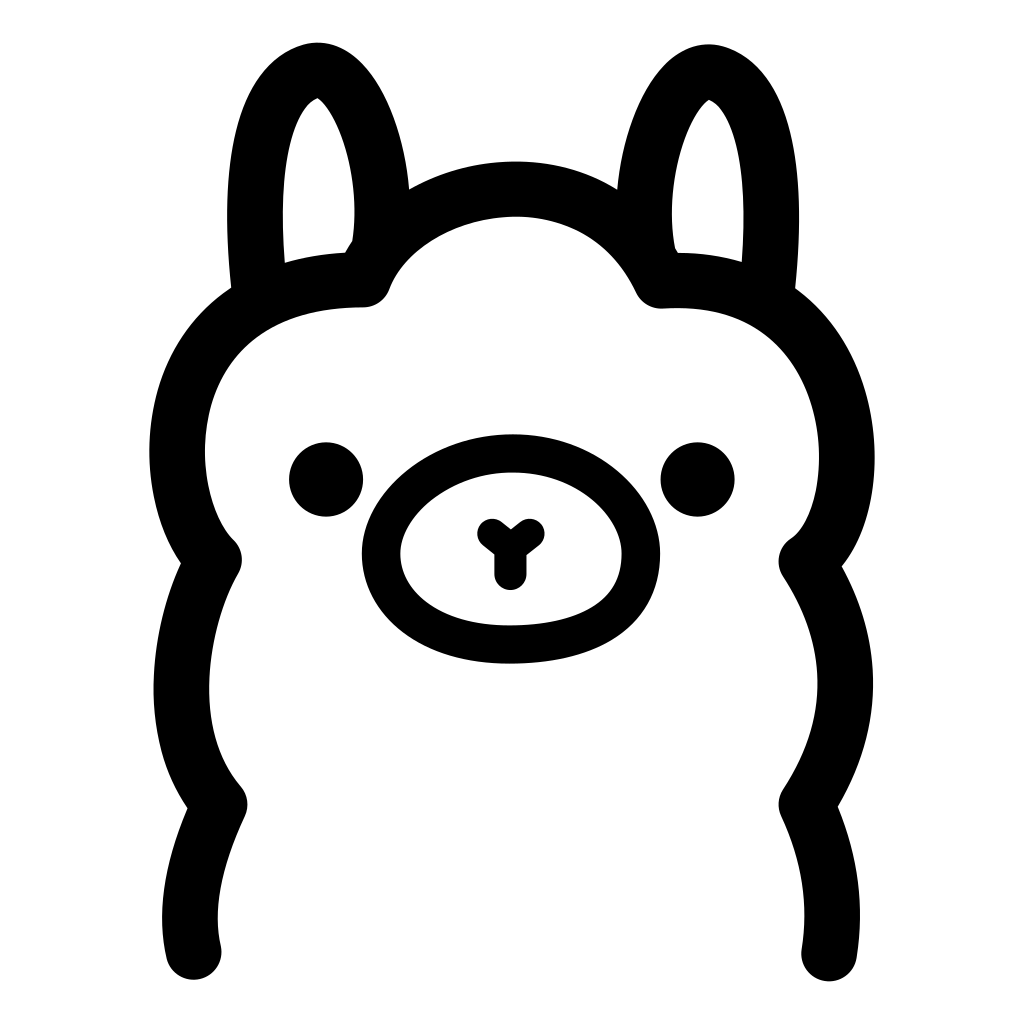
\includegraphics[width=0.2\textwidth, alt={Logo Ollama}]{img/ollama.png}
    \caption[Logo Ollama]{Logo Ollama}\label{fig:logo_ollama}
\end{figure}


\subsection{GitHub}
\label{subsec:github}
\noindent GitHub (logo in figura \ref{fig:logo_github}) è una piattaforma di hosting basata su \glslink{gitg}{Git}, il sistema di controllo di versione distribuito ideato da Linus Torvalds. Lanciata nel 2008, GitHub si è affermata come uno degli strumenti principali per la collaborazione nello sviluppo software, consentendo a sviluppatori di tutto il mondo di condividere, modificare e mantenere progetti in modo coordinato. \\La piattaforma offre funzionalità avanzate per il versionamento del codice, la gestione dei rami (branching), il tracciamento delle modifiche e la revisione collaborativa tramite pull request. \\Oltre a essere uno strumento tecnico, GitHub ha favorito la nascita di una vera e propria comunità \glslink{open-sourceg}{open source}, nella quale il codice è accessibile, riutilizzabile e migliorabile da chiunque.
\begin{figure}[H]
    \centering
    
\includegraphics[width=0.2\textwidth, alt={Logo GitHub}]{img/github.png}
    \caption[Logo GitHub]{Logo GitHub}\label{fig:logo_github}
\end{figure}

\subsection{VSCode}
\label{subsec:vscode}
\noindent Visual Studio Code (logo in figura \ref{fig:logo_vscode}), conosciuto semplicemente come VSCode, è un editor di codice sorgente sviluppato da Microsoft e distribuito gratuitamente. Introdotto nel 2015, ha rapidamente conquistato una posizione di rilievo tra gli strumenti preferiti dagli sviluppatori grazie alla sua combinazione di leggerezza, flessibilità e ricchezza di funzionalità. \\Compatibile con i principali sistemi operativi (Windows, macOS e Linux), VSCode supporta evidenziazione della sintassi per numerosi linguaggi, suggerimenti intelligenti e completamento automatico del codice, strumenti di \glslink{debuggingg}{debugging} integrati e gestione del controllo di versione tramite \glslink{gitg}{Git}. \\Inoltre, grazie a un vasto marketplace di estensioni, può essere facilmente personalizzato per adattarsi a diversi flussi di lavoro e tecnologie, rendendolo un ambiente di sviluppo versatile e ampiamente diffuso.
\begin{figure}[H]
    \centering
    
\includegraphics[width=0.25\textwidth, alt={Logo VSCode}]{img/vscode.jpg}
    \caption[Logo VSCode]{Logo VSCode}\label{fig:logo_vscode}
\end{figure}

\subsection{Total Validator}
\label{subsec:tv}
\noindent Total Validator (logo in figura \ref{fig:logo_TV}) è uno strumento di convalida web che permette di verificare contemporaneamente l’accessibilità secondo le linee guida WCAG 2.0, 2.1 e 2.2, la conformità alla Section 508 statunitense e alle specifiche ARIA. \\Consente inoltre di controllare la validità del codice HTML rispetto a numerosi standard, incluso l’HTML5, e la correttezza dei CSS in conformità con moltwe specifiche del W3C. \\Tra le sue funzioni principali rientrano anche la rilevazione di link interrotti e la verifica ortografica multilingue. Lo strumento permette di analizzare pagine offline, protette da autenticazione o generate dinamicamente tramite JavaScript, risultando così particolarmente flessibile. \\È disponibile per Windows, macOS e Linux e, dal suo lancio nel 2005, è stato adottato da milioni di siti web, comprese istituzioni pubbliche e governative.
\begin{figure}[H]
    \centering
    
\includegraphics[width=0.17\textwidth, alt={Logo Total Validator}]{img/totalvalidator.png}
    \caption[Logo Total Validator]{Logo Total Validator}\label{fig:logo_TV}
\end{figure}

\subsection{WAVE}
\label{subsec:wave}
\noindent WAVE (\textit{Web Accessibility Evaluation Tool}) è uno strumento sviluppato da WebAIM per supportare la valutazione dell’accessibilità dei siti web (logo in figura \ref{fig:logo_wave}). Consente di individuare automaticamente molte violazioni delle WCAG e, al tempo stesso, facilita l’analisi manuale da parte degli sviluppatori.\\ È disponibile come servizio online e come estensione per i principali browser, permettendo di testare anche pagine locali o protette. I risultati vengono visualizzati direttamente sulla pagina tramite icone e pannelli che segnalano errori, avvisi e caratteristiche accessibili, fornendo indicazioni utili per le correzioni. \\Per contesti più complessi, WAVE offre inoltre un’API che ne consente l’integrazione nei processi di sviluppo e di testing automatizzato.
\begin{figure}[H]
    \centering
    
\includegraphics[width=0.2\textwidth, alt={Logo WAVE}]{img/wave.png}
    \caption[Logo WAVE]{Logo WAVE}\label{fig:logo_wave}
\end{figure}

\subsection{Lighthouse}
\label{subsec:lighthouse}
\noindent Lighthouse (logo in figura \ref{fig:logo_lighthouse}) è uno strumento open-source sviluppato da Google per valutare la qualità delle pagine web. Esegue controlli automatici su performance, accessibilità, SEO e progressive web app, restituendo report dettagliati con punteggi e suggerimenti pratici. \\Si può utilizzare tramite Chrome DevTools, riga di comando (CLI), modulo Node o interfaccia web, consentendo anche audit su pagine protette o locali. Lighthouse quindi supporta gli sviluppatori nel miglioramento della velocità di caricamento, dell’usabilità e della visibilità dei siti.
\begin{figure}[H]
    \centering
    
\includegraphics[width=0.17\textwidth, alt={Logo Lighthouse}]{img/lighthouse.png}
    \caption[Logo Lighthouse]{Logo Lighthouse}\label{fig:logo_lighthouse}
\end{figure}
\newpage
    \chapter{Sviluppo}
\label{chap:sviluppo}

\section{Web design}
Il design dell’estensione è stato sviluppato con un approccio desktop-first, in considerazione del target principale costituito da sviluppatori web che operano prevalentemente su schermi di grandi dimensioni. \\Tale scelta consente di privilegiare la chiarezza e l’ampiezza degli spazi di lavoro, garantendo una disposizione ottimale dei pannelli e delle funzionalità principali.\\
\\ %\glslink{desktop-firstg}{\textit{desktop-first}}
Particolare attenzione è stata posta all’accessibilità cromatica, mediante uno studio accurato dei contrasti tra testo, sfondo ed elementi interattivi, al fine di assicurare leggibilità anche in condizioni visive differenti. \\È stata inoltre implementata la possibilità di personalizzare l’esperienza visiva tramite un pulsante dedicato alla selezione della modalità giorno/notte, che permette all’utente di adattare l’interfaccia alle proprie preferenze e alle condizioni ambientali di utilizzo.\\
Nonostante l’approccio iniziale privilegi i dispositivi desktop, il layout rimane responsivo grazie a soluzioni flessibili che mantengono l’usabilità anche su schermi di dimensioni ridotte. Questa scelta assicura un’esperienza coerente ed accessibile in diversi contesti d’uso.

\section{Interazione con l'AI}
L’estensione sviluppata prevede un’integrazione diretta con Ollama. Questa scelta garantisce all’utente il pieno controllo sui dati, riducendo i rischi legati alla trasmissione di informazioni sensibili verso servizi esterni e permettendo un utilizzo anche in assenza di connessione Internet stabile. L’interazione con l’intelligenza artificiale avviene attraverso chiamate HTTP a un endpoint locale, al quale vengono inviati prompt costruiti dinamicamente in base alle esigenze del flusso operativo.

\begin{lstlisting}[language=JavaScript, caption={Funzione di interazione con Ollama}]
async function inviaPrompt(prompt) {
  const res = await fetch('http://localhost:11434/api/generate', {
    method: 'POST',
    headers: { 'Content-Type': 'application/json' },
    body: JSON.stringify({
      model: "llama3.1:8b",
      prompt,
      stream: false
    })
  });
  return await res.json();
}
\end{lstlisting}


Sono stati definiti tre casi d’uso principali per la generazione dei prompt: 
\begin{itemize}
    \item l’invio congiunto del DOM della pagina e della domanda dell’utente, utile per ricevere spiegazioni e indicazioni sulle righe che verranno poi evidenziate in quanto utili alla comprensione della risposta; 
    \begin{lstlisting}[language=JavaScript, caption={Prompt per la generazione di risposta e righe da evidenziare}]
    const promptPrincipale =
    `Sei un assistente che analizza codice HTML. Rispondi alla domanda in modo chiaro ma conciso, usando al massimo 5-6 frasi. ` +
    `Evita ripetizioni o spiegazioni troppo generiche. ` +
    `Alla fine della risposta, su una nuova riga, scrivi le righe eventualmente utilizzate per la risposta nel seguente formato:\n\n` +
    `##RIGHE##\n{"righe": [elenco_di_numeri_di_riga]}\n\n` +
    `Codice HTML:\n${codice}\n\nDomanda: ${domanda}`;
    \end{lstlisting}
    
    \item l'invio della sola domanda per generare ulteriori domande piu' approfondite da consigliare all'utente;
    \begin{lstlisting}[language=JavaScript, caption={Prompt per la generazione di domande successive}]
    const promptSuccessiva =
    `Suggerisci 1 o 2 domande piu' specifiche sull'accessibilita' o sull'analisi del codice, ` +
    `partendo dalla seguente domanda:\n\n` +
    `Rispondi solo con il seguente formato JSON:\n\n` +
    `##DOMANDA##\n{ "domande": ["prima domanda", "seconda...", "terza..."] }\n\n` +
    `Domanda iniziale: ${domanda}`;
    \end{lstlisting}

    
    \item l’invio del DOM insieme alla richiesta di modifica, scenario in cui l’IA produce sia una risposta argomentata sia un blocco di codice pronto per essere inserito nel pannello centrale della pagina nella modalità di sviluppo guidato.
    \begin{lstlisting}[language=JavaScript, caption={Prompt per la generazione di risposta e codice html accessibile}]
    const promptCodice =
      `Sei un assistente che aiuta a rendere accessibile il codice HTML. ` +
      `Rispondi in massimo 5-6 frasi chiare e tecniche. ` +
      `Se suggerisci del codice, racchiudilo tra i marcatori \`##CODICE##\` come mostrato di seguito:\n\n` +
      `##CODICE##\n<codice HTML da inserire o modificare>\n##FINECODICE##\n\n` +
      `Codice HTML:\n${codice}\n\nDomanda: ${domanda}`;
    \end{lstlisting}

\end{itemize}
Questa diversificazione consente di mantenere un approccio modulare e adattabile, rendendo l’assistente in grado di rispondere a necessità differenti con un unico modello sottostante.


\section{Filtraggio risposta generata}
Un aspetto fondamentale del funzionamento dell'estensione riguarda il filtraggio e la rielaborazione della risposta generata dall’intelligenza artificiale. Le risposte restituite da Ollama, infatti, non vengono mostrate direttamente all’utente, ma sono sottoposte ad un processo di parsing e di pulizia.\\
In primo luogo, l’estensione distingue le diverse tipologie di output attese: la risposta vera e propria alla domanda inserita, le eventuali domande suggerite e gli eventuali blocchi di codice generati da visualizzare e/o scaricare. A tal fine vengono utilizzati marcatori testuali inseriti nel prompt (ad esempio \texttt{\#\#DOMANDE\#\#} o \texttt{\#\#CODICE\#\#}), che consentono di individuare con precisione le sezioni rilevanti all’interno della risposta. \\Una volta ricevuto l’output, funzioni dedicate come \texttt{estraiRigheDaRisposta} ed \texttt{estraiDomandeSuggerite} applicano espressioni regolari per isolare le parti utili, scartando elementi ridondanti o formattazioni non necessarie.\\
\\
Il filtraggio consente anche di separare le informazioni in blocchi distinti, in modo che ciascun contenuto possa essere mostrato nella pagina web nel pannello appropriato (ad esempio, suggerimenti testuali nella chat e codice sorgente nel riquadro centrale). Questo approccio riduce il carico cognitivo per l’utente, che non si trova di fronte a una risposta grezza e complessa, ma ad un output strutturato e facilmente navigabile.\\ Inoltre la possibilità di visualizzare alcune righe di codice evidenziate consente una comprensione più immediata del codice sorgente analizzato rendendo più intuitivo il processo di revisione del codice.
    \definecolor{emerald}{RGB}{0, 168, 107}
\definecolor{darkblue}{RGB}{0,0,139}

\hypersetup{
  colorlinks=true,
  linkcolor=blue,   % sezioni, figure, tabelle in blu
  citecolor=blue,   % bibliografia
  urlcolor=darkblue  % link esterni
}

\DeclareRobustCommand{\wcagref}[2][]{%
  \hyperref[#1]{\textcolor{emerald}{#2}}%
}

\chapter{Test}
\label{chap:test}

\section{Test ``Analisi assistita''}
\noindent Per effettuare i test dell’estensione sono stati utilizzati alcuni siti realizzati per l'edizione 2025 del concorso \textit{Accattivante Accessibile}.\
I test hanno preso in considerazione gli errori individuati da TV insieme a quelli segnalati dalla docente referente e sono stati messi a confronto con gli errori rilevati da \textit{SviluppAbile}.
Infine, ho confrontato i risultati elaborando un resoconto tabellare per ciascun sito analizzato e, successivamente, ho applicato la metrica F\textsubscript{1}-score per ottenere un report oggettivo.

\subsection{F1-score}
\noindent La F\textsubscript{1}-score è una metrica utilizzata per valutare modelli di classificazione, sia binari che multi‐classe. Essa combina in un unico valore la \textit{precision} (quanto le predizioni positive sono corrette) e il \textit{recall} (quanti casi positivi reali vengono identificati), calcolati come:

\[
\text{Precision} = \frac{TP}{TP + FP}, 
\qquad
\text{Recall} = \frac{TP}{TP + FN}
\]

\vspace{0.5cm}
\noindent L’F\textsubscript{1}-score è definita come la media armonica di tali valori:

\[
F_{1} = 2 \cdot \frac{\text{Precision} \cdot \text{Recall}}{\text{Precision} + \text{Recall}}
 = \frac{2 \cdot TP}{2 \cdot TP + FP + FN}
\]
\vspace{0.1cm}

\noindent Questo significa che nel calcolo verranno utilizzati i tre dati rilevati nel presente lavoro:
"errori trovati" come \(TP\) (veri positivi), "errori non trovati" come \(FN\) (falsi negativi), e \(FP\) (falsi positivi).
In questo modo, l’F\textsubscript{1}-score riflette in modo equilibrato sia la capacità di individuare correttamente errori reali, sia il controllo sui falsi allarmi.\\

\noindent L’F\textsubscript{1}-score assume valori compresi tra 0 e 1. Il valore minimo, \(0\), indica prestazioni pessime (almeno una delle due metriche è nulla), mentre il valore massimo, \(1\), corrisponde a prestazioni perfette (precisione e recall entrambi pari a 1).\\
Valori prossimi a 1 indicano quindi un buon funzionamento del sistema, mentre valori vicini a 0 segnalano performance insoddisfacenti.


% SUDOKU WORLD
\subsection{Sito web: SudokuWorld}
\noindent Di seguito vengono riportati alcuni dei test effettuati sul sito \href{https://caa.studenti.math.unipd.it/amonaco/Sudokuworld/pages/home.php}{SudokuWorld}.

\subsubsection{Total Validator}
\begin{figure}[H]
    \centering
    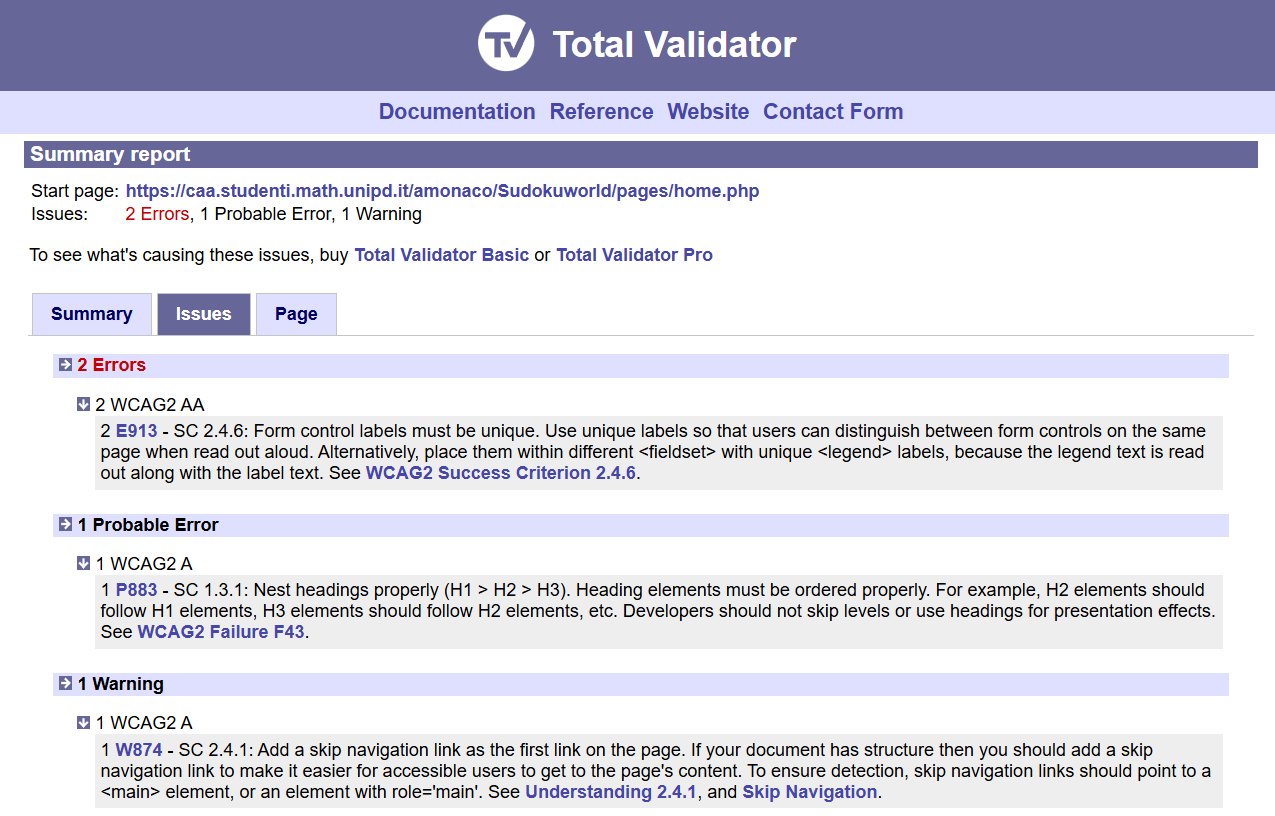
\includegraphics[width=0.7\linewidth, alt={Screenshot dell'analisi di Total Validator sul sito web SudokuWorld}]{img/TV_sudoku.png}
    \caption{Analisi di Total Validator sul sito web \textit{SudokuWorld}}\label{fig:TV_sudoku}
\end{figure}

\noindent L'analisi (vedi figura \ref{fig:TV_sudoku}) ha evidenziato due errori principali: etichette dei controlli dei form non univoche e intestazioni nidificate in modo non corretto. 
È stato inoltre segnalato un warning relativo all’assenza di un link di navigazione rapida. 
 
\subsubsection{Lighthouse}
\noindent Il report generato dallo strumento Lighthouse ha restituito un punteggio di 100/100 nella sezione Accessibility, indicando che, secondo le metriche automatiche adottate, non sono stati rilevati errori o problematiche di conformità (vedi figura \ref{fig:Lighthouse_sudoku}).
\begin{figure}[H]
    \centering
    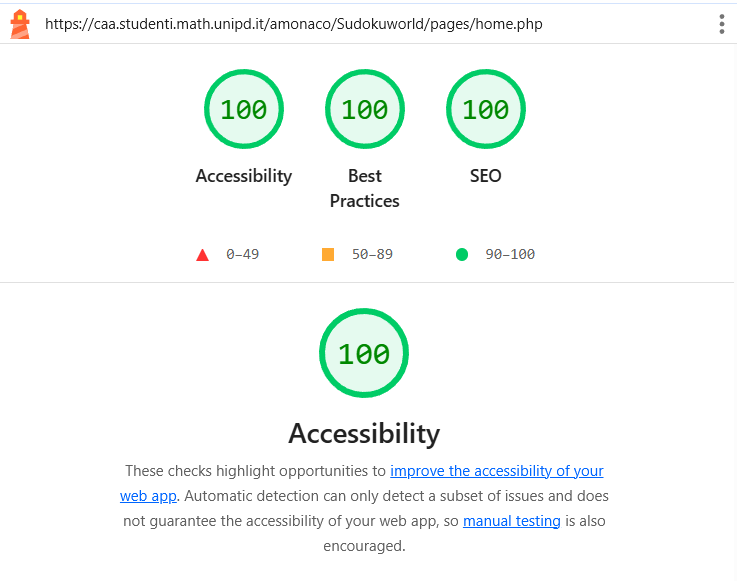
\includegraphics[width=0.6\linewidth, alt={Screenshot dell'analisi di Lighthouse sul sito web SudokuWorld}]{img/Lighthouse_sudoku.png}
    \caption{Analisi di Lighthouse sul sito web \textit{SudokuWorld}}\label{fig:Lighthouse_sudoku}
\end{figure}

\subsubsection{SviluppAbile}
\noindent Di seguito vengono riportati alcuni esempi di domande poste all’estensione \textit{SviluppAbile} e delle relative risposte ricevute. \newline
\\ \vspace{-0.5cm}
\noindent(pagina home.php)\\
\subsubsection*{\texttt{Il mio codice HTML rispetta le linee guida WCAG?}}
\begin{adjustwidth}{1cm}{1cm}
\noindent {\footnotesize Il tuo codice HTML sembra essere in parte conforme alle linee guida WCAG (Web Content Accessibility Guidelines), ma potrebbe migliorare ulteriormente per garantire una maggiore accessibilità. Alcune aree che richiedono ulteriore attenzione includono:\\
- L'attributo `aria-label` non è utilizzato in modo coerente nei controlli di navigazione.\\
- Le etichette dei pulsanti "Cerca" e "Profilo" potrebbero essere più descrittive.\\
Tuttavia, il tuo codice include molti elementi positivi come l'utilizzo di `alt` per immagini, la presenza di un titolo (`<title>`) e di metatag di descrizione (`<meta name="description">`). Questi sono passaggi fondamentali per migliorare la comprensione del contenuto da parte dei motori di ricerca e degli assistenti.\\
Per garantire una maggiore accessibilità, considera di applicare ulteriormente le linee guida WCAG 2.1, che offrono standard e raccomandazioni per creare esperienze web più inclusive.\\
La pagina non rispetta la norma W3C WCAG 2.1 che richiede di nidificare correttamente le intestazioni. Non sono presenti elementi HTML con attributo "h1", mentre ci sono intestazioni con grado inferiore.\\
La situazione descritta viola la regola WCAG 1.3.1, che richiede la corretta gerarchia di intestazioni (H1 > H2 > H3). In questo caso, l'h2 non è diretto al figlio dell'H1.\\
Vi è inoltre la presenza di due etichette (label) con il valore "Cerca" all'interno della stessa pagina HTML, ma con attributi id diversi ("searched-product" e "for"). Secondo la specifica SC 2.4.6, le etichette dei form control devono essere uniche.
}
\end{adjustwidth}

\subsubsection*{\texttt{Vi sono errori riguardanti i link?}}
\begin{adjustwidth}{1cm}{1cm}
\noindent {\footnotesize Il codice HTML contiene due carousel circolari:\\
1.  Il primo è definito come "specialProductsCarousel" e si trova nella sezione `<main>`.\\
2.  Il secondo è chiamato "bestSellersCarousel" ed è anch'esso presente all'interno della stessa sezione.\\
Quanto ai controlli sui link visitati, non sono implementati controlli specifici per la traccia dei link visitati sul sito web.
} \\
\end{adjustwidth}

\noindent(pagina sudoku.php)
\vspace{-0.5cm}
\subsubsection*{\texttt{Il mio codice HTML rispetta le linee guida WCAG?}} 
\begin{adjustwidth}{1cm}{1cm}
\noindent {\footnotesize Il tuo codice HTML non rispetta pienamente le linee guida WCAG (Web Content Accessibility Guidelines) per diverse ragioni:\\
1.  **La navigazione è troppo complessa**: la barra di navigazione contiene molti elementi e link, potrebbe essere difficile per gli utenti disabili utilizzare l'interfaccia.\\
2.  **L'accessibilità dei form è insufficiente**: non sono presenti attributi accessibili per i campi di input e submit, rendendo la navigazione dei form difficoltosa per gli utenti che usano dispositivi di assistenza.\\
3.  **La lettura dei testi in basso risulta difficile**: alcuni elementi come il timer sono troppo piccoli per essere letti facilmente dagli schermi con alto contrasto o da dispositivi di assistenza.\\
4.  **Non ci sono alternative al linguaggio naturale**: le immagini contengono solo icone e simboli, che potrebbero non essere compresi da utenti analfabetici.\\
\\Aggiungere attributi accessibili ai campi input e submit:\\
*   Modifica il codice HTML come segue:\\
    \texttt{<form class="d-flex align-items-center my-2 my-lg-0 ms-auto" \\ action="/amonaco/Sudokuworld/pages/search.php" method="GET"> 
    \begin{adjustwidth}{1cm}{}  <label for="searched-product" class="visually-hidden">Cerca</label>\end{adjustwidth}
    \begin{adjustwidth}{1cm}{} 
        <input class="form-control me-2" type="search" name="searched-product" id="searched-product" placeholder="Cerca" value="" aria-label="Search" />
    \end{adjustwidth}
    \begin{adjustwidth}{1cm}{} 
        <button class="btn btn-outline-success" type="submit" \textbf{aria-label="Submit the form"}>Cerca</button>
    \end{adjustwidth}
    </form>}\\
\\Aggiungere tag alt alle immagini: assicurati di aggiungere il contenuto alternativo per ogni immagine.\\
*   Modifica il codice HTML come segue:\\
    \texttt{<a class="nav-link" href="/amonaco/Sudokuworld/pages/sudoku.php">\\
    \indent <i class="bi bi-grid-3x3-gap-fill"></i>\\
    </a>}\\
\\Aggiungere tag aria: per fornire informazioni aggiuntive alle pagine web, puoi utilizzare gli attributi aria.\\
*   Modifica il codice HTML come segue:\\
    \texttt{<h1 class="container border border-black p-2 mb-4 rounded text-center" id="sudokuTitle" role="heading" aria-level="1">!! Sudoku !!</h1>}\\
\\Controlla l'accessibilità con strumenti di testing: prima della pubblicazione, assicurati di utilizzare strumenti come Lighthouse o WAVE per valutare la tua pagina web e risolvere eventuali problemi.\\
Ricorda che un sito web accessibile è più facile da utilizzare per tutti gli utenti, compresi quelli con disabilità.\\
\\
\texttt{DOMANDE SUGGERITE: \\"Quale è il criterio WCAG 2.1 che riguarda la navigazione con tastiera?"
\\"Come posso utilizzare gli strumenti di analisi del codice per identificare le aree dell'accessibilità da migliorare nel mio sito web HTML?"
}}
\end{adjustwidth}

\paragraph*{\texttt{"Come posso utilizzare gli strumenti di analisi del codice per \\ identificare le aree dell'accessibilità da migliorare nel mio sito web HTML?"}} 
\begin{adjustwidth}{1cm}{1cm}
\noindent {\footnotesize Per identificare le aree dell'accessibilità da migliorare nel tuo sito web HTML, puoi utilizzare gli strumenti di analisi come W3C Validator e Lighthouse. Il W3C Validator verifica la correttezza del codice HTML e fornisce suggerimenti per migliorare l'accessibilità. Lighthouse è uno strumento open-source che valuta l'accessibilità, le prestazioni e la sicurezza del tuo sito web.}
\end{adjustwidth}

\vspace{0.8cm}

\noindent \textbf{Resoconto finale dei test}\\
\noindent Di seguito viene illustrato il processo di test effettuato da \textit{SviluppAbile} confrontando i risultati ottenuti dagli altri strumenti di validazione e integrando anche un controllo manuale basato sulle Web Content Accessibility Guidelines (WCAG 2.1). Lo studio è stato articolato sulle principali pagine del sito, inclusa l’area riservata.\\

\noindent \textbf{Pagina home.php}\\
L’estensione \textit{SviluppAbile} ha rilevato la mancanza di una gerarchia corretta delle intestazioni: non è presente un elemento <h1>, mentre compaiono direttamente intestazioni di livello inferiore. Questo comportamento viola il criterio {\wcagref[wcag:1.3.1]{\textit{1.3.1 - Info and Relationships}}}, che prescrive una corretta nidificazione semantica. Inoltre, sono state individuate etichette duplicate per i campi di ricerca, contrarie al criterio {\wcagref[wcag:2.4.6]{\textit{2.4.6 - Headings and Labels}}}, ed un utilizzo incoerente di aria-label nei controlli di navigazione, che può generare confusione negli screenreader.
L’analisi manuale ha permesso di osservare ulteriori criticità, tra cui la mancanza di un meccanismo di bypass (skip link) in violazione del criterio {\wcagref[wcag:2.4.1]{\textit{2.4.1 - Bypass Blocks}}}.\\

\noindent \textbf{Pagina sudoku.php}\\
In questa pagina è stato rilevato che i form risultano privi di etichette accessibili e che i pulsanti non sono sufficientemente descrittivi, in contrasto con i criteri {\wcagref[wcag:3.3.2]{\textit{3.3.2 - Labels or Instructions}}} e {\wcagref[wcag:4.1.2]{\textit{4.1.2 - Name, Role, Value}}}. È stata inoltre segnalata l’assenza di testi alternativi per le icone, che viola il criterio {\wcagref[wcag:1.1.1]{\textit{1.1.1 - Non-text Content}}}. Alcuni elementi testuali, come il timer, presentano dimensioni ridotte e difficilmente leggibili, con possibili ricadute sul criterio {\wcagref[wcag:1.4.4]{\textit{1.4.4 - Resize Text}}}.
Un’osservazione manuale ha evidenziato che i contrasti cromatici non sempre soddisfano il rapporto minimo richiesto dal criterio {\wcagref[wcag:1.4.3]{\textit{1.4.3 - Contrast (Minimum)}}} e che non è garantita la piena navigabilità da tastiera ({\wcagref[wcag:2.1.1]{\textit{2.1.1}}}).\\

\noindent \textbf{Pagina search.php}\\
La pagina di ricerca consente agli utenti di filtrare e visualizzare i prodotti disponibili. 
L’estensione \textit{SviluppAbile} ha rilevato alcune criticità principali: assenza di intestazione <h1>, che viola il criterio {\wcagref[wcag:1.3.1]{\textit{1.3.1}}}, etichette duplicate nei campi di ricerca ({\wcagref[wcag:2.4.6]{\textit{2.4.6}}}) e uso incoerente di aria-label nei controlli di navigazione.\\
L’analisi tramite strumenti di accessibilità ha evidenziato ulteriori problematiche: mancata navigabilità completa da tastiera ({\wcagref[wcag:2.1.1]{\textit{2.1.1}}}), testi alternativi mancanti per le icone o immagini illustrative ({\wcagref[wcag:1.1.1]{\textit{1.1.1}}}) e che il contrasto di alcuni elementi testuali non soddisfa il rapporto minimo previsto ({\wcagref[wcag:1.4.3]{\textit{1.4.3}}}).\\

\noindent \textbf{Pagine product.php?id=…}\\
Le schede prodotto (analizzando quelle relative alla tazza “I love sudoku” e alla maglia “commit sudoku”) hanno mostrato ulteriori problematiche. \textit{SviluppAbile} ha rilevato la mancanza di testi alternativi per le immagini ({\wcagref[wcag:1.1.1]{\textit{1.1.1}}}), l’assenza di titoli significativi nei tag <title> ({\wcagref[wcag:2.4.2]{\textit{2.4.2 - Page Titled}}}) e l’utilizzo non semantico del markup per i prezzi scontati ({\wcagref[wcag:1.3.1]{\textit{1.3.1}}}). Sono stati inoltre segnalati link privi di indicazioni chiare di stato focus o visited ({\wcagref[wcag:2.4.7]{\textit{2.4.7 - Focus Visible}}}) e la mancanza di attributi ARIA utili a descrivere pulsanti generici come “Aggiungi al carrello” ({\wcagref[wcag:4.1.2]{\textit{4.1.2}}}). Ques'ultimo errore rappresenta un falso negativo, in quanto il pulsante è definito correttamente.
L’analisi tramite strumenti di accessibilità ha messo in luce ulteriori difetti: contrasti di colore insufficienti ({\wcagref[wcag:1.4.3]{\textit{1.4.3}}}), assenza di skip link ({\wcagref[wcag:2.4.1]{\textit{2.4.1}}}) e mancanza di landmark semantici ({\wcagref[wcag:1.3.1]{\textit{1.3.1}}}).\\

\noindent \textbf{Pagina carrello.php}\\
Sebbene l’estensione non abbia segnalato particolari criticità nella struttura della pagina, un’analisi manuale rivela che i prodotti nel carrello non sono accompagnati da testi alternativi adeguati per le immagini ({\wcagref[wcag:1.1.1]{\textit{1.1.1}}}), né da descrizioni sufficientemente univoche per i pulsanti di azione, come “Rimuovi” o “Procedi al pagamento”. La mancanza di etichette descrittive viola i criteri {\wcagref[wcag:2.4.6]{\textit{2.4.6}}} e {\wcagref[wcag:3.3.2]{\textit{3.3.2}}}.\\

\noindent \textbf{Pagina login.php}\\
L’accesso alla pagina di login con credenziali di test ha permesso all'estensioene di segnalare alcune criticità: i campi di input risultano privi di etichette esplicite e i pulsanti sono generici, compromettendo la fruibilità per chi utilizza tecnologie assistive ({\wcagref[wcag:3.3.2]{\textit{3.3.2}}} e {\wcagref[wcag:4.1.2]{\textit{4.1.2}}}). Inoltre viene segnalata l'assenza di attributi \texttt{aria-label} sui controlli di autenticazione. Quest'ultimo errore in realtà è un falso negativo, derivante dalla capacità ridotta di analisi dell'IA alla base dell'estensione.\\
L’analisi manuale ha messo in luce ulteriori problematiche non rilevate dallo strumento: la mancanza di messaggi di errore in caso di inserimento di credenziali errate ({\wcagref[wcag:3.3.1]{\textit{3.3.1 - Error Identification}}}), link come “Registrati” privi di testo descrittivo contestuale ({\wcagref[wcag:2.4.4]{\textit{2.4.4 - Link Purpose (In Context)}}}), e la mancanza di informazioni semantiche aggiuntive che faciliterebbero la navigazione da tastiera ({\wcagref[wcag:2.1.1]{\textit{2.1.1}}}). \\

\noindent \textbf{Conclusioni}\\
Il confronto tra i risultati di \textit{SviluppAbile} e l’analisi tramite strumenti di convalida (integrata con un'analisi manuale) basati sulle WCAG mostra come l’estensione sia efficace nell’individuare errori comuni e strutturali – quali la mancanza di testi alternativi, etichette duplicate, heading disordinati e pulsanti privi di descrizione – ma non riesca a rilevare altri aspetti fondamentali per l’accessibilità, come i contrasti cromatici e la presenza di skip link. Inoltre l'estensione suggerisce modifiche non conformi, come ad esempio attributi alt non idonei.\\
Questo dimostra che uno strumento automatico, pur costituendo un valido supporto, deve al giorno d'oggi ancora essere integrato con una verifica manuale alla luce delle linee guida ufficiali del W3C.

\paragraph{F1-score} \mbox{}\\
\noindent Nella tabella \ref{tab:sudokuWorld} vengono riassunti i risultati ottenuti.
\begin{footnotesize}
\begin{longtable}[c]{|C{4.8cm}|C{4.8cm}|C{4.8cm}|}
\caption{Tabella riassuntiva analisi \textit{SudokuWorld} tramite \textit{SviluppAbile}}
\label{tab:sudokuWorld}\\
\hline
\textbf{Errori trovati} & \textbf{Errori non trovati} & \textbf{Falsi positivi}\\
\hline
\endfirsthead
\multicolumn{3}{c}%
{{\bfseries Tabella \thetable\ -- continua dalla pagina precedente}} \\
\hline
\textbf{Errori trovati} & \textbf{Errori non trovati} & \textbf{Falsi positivi}\\
\hline
\endhead
\hline
\multicolumn{3}{r}{{ -- continua nella pagina successiva}} \\
\endfoot
\hline
\endlastfoot
\begin{itemize}
    \item h1 > h2 > h3
    \item Etichette dei form non univoche
    \item Errori con gli alt
    \item Errore button "registrati" 
    \item Link circolari
    \item Manca controllo link già visitati 
\end{itemize}
 & \begin{itemize}
    \item Contrasti dei colori
    \item Skip navigation link
\end{itemize}
 & \begin{itemize}
    \item Tag ARIA (suggerimenti errati)
    \item Suggerimenti alt errati
\end{itemize}\\
\hhline{|=|=|=|} 
6 & 2 & 2 \\
\end{longtable}
\end{footnotesize}

\noindent L'F\textsubscript{1}-score calcolato è $F_{1}=0.75$, un valore piuttosto buono che indica una capacità complessiva soddisfacente di individuare gli errori reali, pur con la presenza di alcuni mancati rilevamenti e di falsi positivi. 
Ciò suggerisce che l’estensione riesce a fornire risultati utili e affidabili, anche se rimane margine per ulteriori miglioramenti nella precisione e nella completezza dell’analisi.

% === DOLCE RISVEGLIO ===
\subsection{Sito web: Dolce Risveglio}
\noindent Di seguito vengono riportati alcuni dei test effettuati sul sito web \href{https://caa.studenti.math.unipd.it/gchecchi/}{Dolce Risveglio}.

\subsubsection{Total Validator}
\begin{figure}[H]
    \centering
    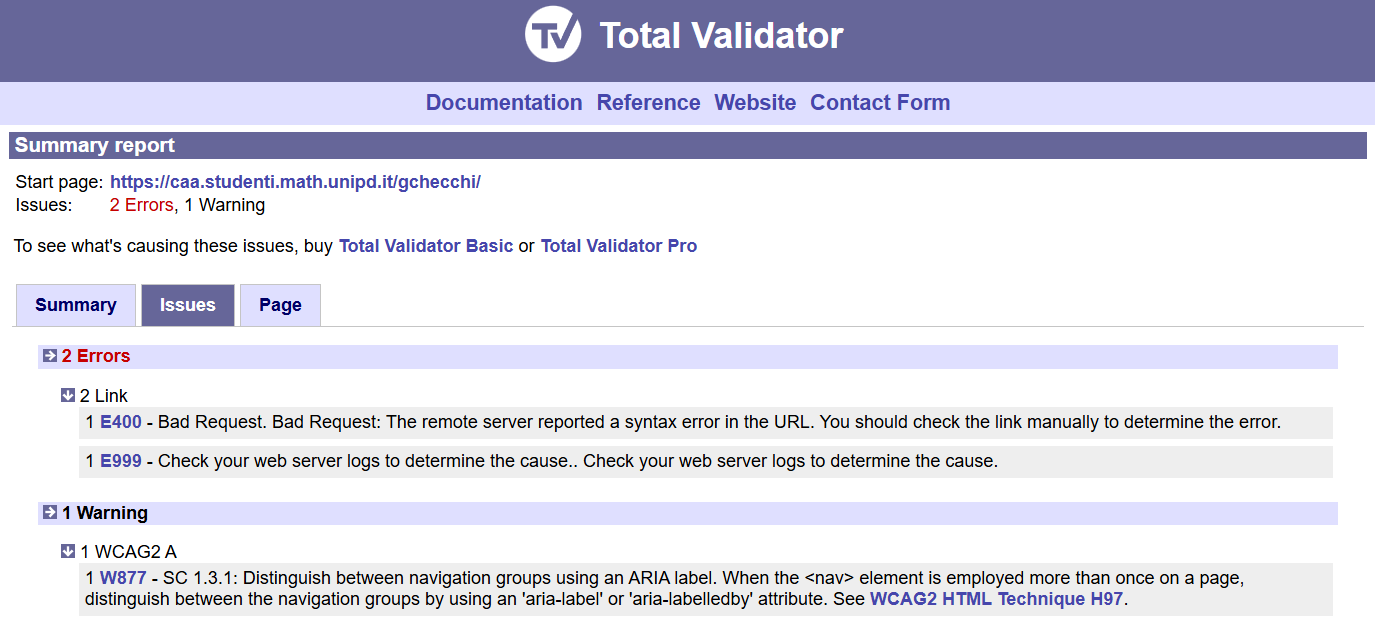
\includegraphics[width=0.9\linewidth, alt={Screenshot dell'analisi di Total Validator sul sito web Dolce Risveglio}]{img/TV_dolcerisveglio.png}
    \caption{Analisi di Total Validator sul sito web \textit{Dolce Risveglio}}\label{fig:TV_dolcerisveglio}
\end{figure}

\noindent L'analisi (vedi figura \ref{fig:TV_dolcerisveglio}) ha rilevato 2 errori relativi ai link e 1 warning. 
Gli errori comprendono un URL con richiesta non valida e un problema lato server da verificare nei log. 
Il warning riguarda la necessità di distinguere tra più aree di navigazione tramite un'etichetta ARIA. 

\subsubsection{Lighthouse}
\noindent Il report ha restituito un punteggio di 100/100 nella sezione \textit{Accessibility}, indicando che, secondo le metriche automatiche adottate, non sono stati rilevati errori o problematiche di conformità (vedi figura \ref{fig:Lighthouse_dolcerisveglio}).
\begin{figure}[H]
    \centering
    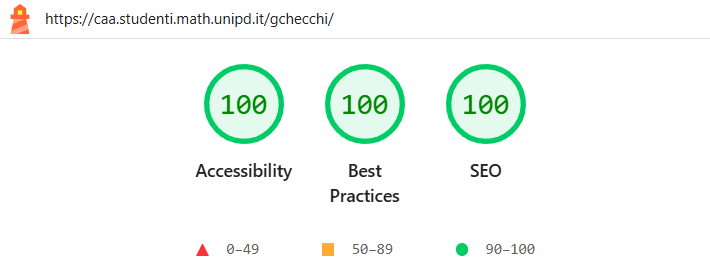
\includegraphics[width=0.6\linewidth, alt={Screenshot dell'analisi di Lighthouse sul sito web DolceRisveglio}]{img/Lighthouse_dolcerisveglio.png}
    \caption{Analisi di Lighthouse sul sito web \textit{Dolce Risveglio}}\label{fig:Lighthouse_dolcerisveglio}
\end{figure}

\subsubsection{Sviluppabile}
\noindent Di seguito viene illustrato il processo di test effettuato da \textit{SviluppAbile} confrontando i risultati ottenuti dagli altri strumenti di validazione e integrando anche un controllo manuale basato sulle Web Content Accessibility Guidelines (WCAG 2.1). Lo studio è stato articolato sulle principali pagine del sito.\\

\noindent \textbf{Pagina home.php}\\
La pagina presenta una panoramica della caffetteria, con sezioni dedicate alla storia del locale, ai prodotti offerti e link al menù. L’estensione ha rilevato alcune criticità principali: immagini prive di testi alternativi ({\wcagref[wcag:1.1.1]{\textit{1.1.1 - Non-text Content}}}), uso di intestazioni senza gerarchia coerente ({\wcagref[wcag:1.3.1]{\textit{1.3.1 - Info and Relationships}}}) e suggerimenti per aggiungere label ed id negli elementi di input ({\wcagref[wcag:2.4.6]{\textit{2.4.6 - Headings and Labels}}}).\\
L’analisi tramite strumenti automatici ha evidenziato ulteriori problemi: contrasto insufficiente in alcune aree di testo o link ({\wcagref[wcag:1.4.3]{\textit{1.4.3}}}) e l'assenza di alcuni alt ({\wcagref[wcag:1.1.1]{\textit{1.1.1}}}).\\

\noindent \textbf{Pagina menu.php}\\
La pagina presenta il menù della caffetteria, con sezioni dedicate a bevande, pietanze e dolci, strutturate in liste e tabelle descrittive (\texttt{<dl>}). 
L’estensione \textit{SviluppAbile} ha rilevato alcune criticità principali: immagini dei piatti prive di testi alternativi significativi ({\wcagref[wcag:1.1.1]{\textit{1.1.1}}}), bottoni per la selezione dei menu senza chiara indicazione dello stato attivo tramite attributi ARIA ({\wcagref[wcag:4.1.2]{\textit{4.1.2 - Name, Role, Value}}}) e suggerimenti per aggiungere label agli elementi interattivi ({\wcagref[wcag:2.4.6]{\textit{2.4.6}}}). L'estensione suggerisce inoltre una modifica delle tabelle descrittive; tale modifica è purtroppo errata in quanto l'IA attualmente non è in grado di creare correttamente tabelle accessibili.\\
Ulteriori controlli con strumenti automatici hanno evidenziato problemi come contrasti insufficienti tra testo e sfondo in alcune aree del menù ({\wcagref[wcag:1.4.3]{\textit{1.4.3}}}) e assenza di skip link funzionanti per navigare rapidamente tra le sezioni del menù ({\wcagref[wcag:2.4.1]{\textit{2.4.1}}}).\\

\noindent \textbf{Pagina contatti.php}\\
La pagina consente agli utenti di inviare richieste o informazioni tramite un modulo di contatto, presentando campi per nome, email, telefono e messaggio. L’estensione ha rilevato alcune criticità principali: immagini con alt poco chiari ({\wcagref[wcag:1.1.1]{1.1.1}}), campi del modulo senza indicazioni ARIA aggiuntive per facilitare la navigazione e la comprensione ({\wcagref[wcag:4.1.2]{\textit{4.1.2}}}) e suggerimenti per aggiungere label più descrittive agli elementi interattivi presenti nel footer ({\wcagref[wcag:2.4.6]{\textit{2.4.6}}}).\\
L’analisi tramite strumenti automatici ha evidenziato ulteriori problemi: contrasto insufficiente tra testo e sfondo in alcune aree ({\wcagref[wcag:1.4.3]{\textit{1.4.3}}}), assenza di landmark semantici principali (\texttt{<main>} e \texttt{<nav>}) ({\wcagref[wcag:1.3.1]{\textit{1.3.1}}}) e mancanza di skip link alternativi per navigare rapidamente al contenuto principale ({\wcagref[wcag:2.4.1]{\textit{2.4.1}}}).\\

\noindent \textbf{Pagina prenotazioni.php}\\
La pagina \texttt{prenotazioni.php} permette agli utenti di prenotare un tavolo, specificando nome, email, telefono, giorno, orario e tavolo desiderato tramite un modulo strutturato. L’estensione ha rilevato alcune criticità principali: immagini prive di testi alternativi ({\wcagref[wcag:1.1.1]{\textit{1.1.1}}}), campi del modulo senza indicazioni ARIA aggiuntive per facilitare la comprensione e l’interazione ({\wcagref[wcag:4.1.2]{\textit{4.1.2}}}) e un errore riguardante l'uso improprio degli attributi required e aria-required nello stesso tag, che può genereare errori.\\
L’analisi tramite strumenti automatici non ha evidenziato ulteriori problemi.\\

\noindent \textbf{Conclusioni}\\
Il confronto tra i risultati di \textit{SviluppAbile} e le verifiche effettuate con strumenti automatici mostra che l’estensione è efficace nell’individuare errori di struttura e contenuto, come testi alternativi mancanti, etichette non descrittive e incongruenze tra attributi \texttt{required} e \texttt{aria-required}. Tuttavia, l’estensione non rileva completamente problematiche relative al contrasto cromatico, landmark semantici, skip link e piena navigabilità da tastiera.\\
Per ottenere una valutazione completa dell’accessibilità del sito, è necessario integrare l’uso di \textit{SviluppAbile} con controlli aggiuntivi basati sulle WCAG, assicurando che tutti i form abbiano label univoche, id coerenti e indicazioni ARIA appropriate.


\paragraph{F1-score} \mbox{}\\
\noindent Nella tabella \ref{tab:dolcerisveglio} vengono riportati i risultati ottenuti utilizzando l'estensione \textit{SviluppAbile}.
\begin{footnotesize}
\begin{longtable}[c]{|C{4.8cm}|C{4.8cm}|C{4.8cm}|}
\caption{Tabella riassuntiva analisi \textit{Dolce Risveglio} tramite \textit{SviluppAbile}}
\label{tab:dolcerisveglio}\\
\hline
\textbf{Errori trovati} & \textbf{Errori non trovati} & \textbf{Falsi positivi}\\
\hline
\endfirsthead
\multicolumn{3}{c}%
{{\bfseries Tabella \thetable\ -- continua dalla pagina precedente}} \\
\hline
\textbf{Errori trovati} & \textbf{Errori non trovati} & \textbf{Falsi positivi}\\
\hline
\endhead
\hline
\multicolumn{3}{r}{{ -- continua nella pagina successiva}} \\
\endfoot
\hline
\endlastfoot
\begin{itemize}
    \item Alt non corretti delle img
    \item Etichette dei form non univoche
    \item Suggerisce l'aggiunta di label e id per gli elementi input
    \item Errore required e aria-required utilizzati insieme
\end{itemize}
 & 
\begin{itemize}
    \item Alcuni alt mancanti
\end{itemize}
 & \begin{itemize}
    \item Suggerisce un eccessivo uso di ARIA
\end{itemize}\\
\hhline{|=|=|=|} 
4 & 1 & 1 \\
\end{longtable}
\end{footnotesize}

\noindent L'F\textsubscript{1}-score calcolato è $F_{1}=0.8$, un risultato positivo che evidenzia una buona capacità di individuazione degli errori effettivi, con un numero limitato di falsi positivi e pochi elementi mancati.

% === E-LIXIRIUM ===
\subsection{Sito web: E-lixirium}
\noindent Di seguito vengono riportati alcuni dei test effettuati sul sito web \href{https://caa.studenti.math.unipd.it/abaldazz/?page=home}{E-lixirium}.
\subsubsection{Total Validator}
\begin{figure}[H]
    \centering
    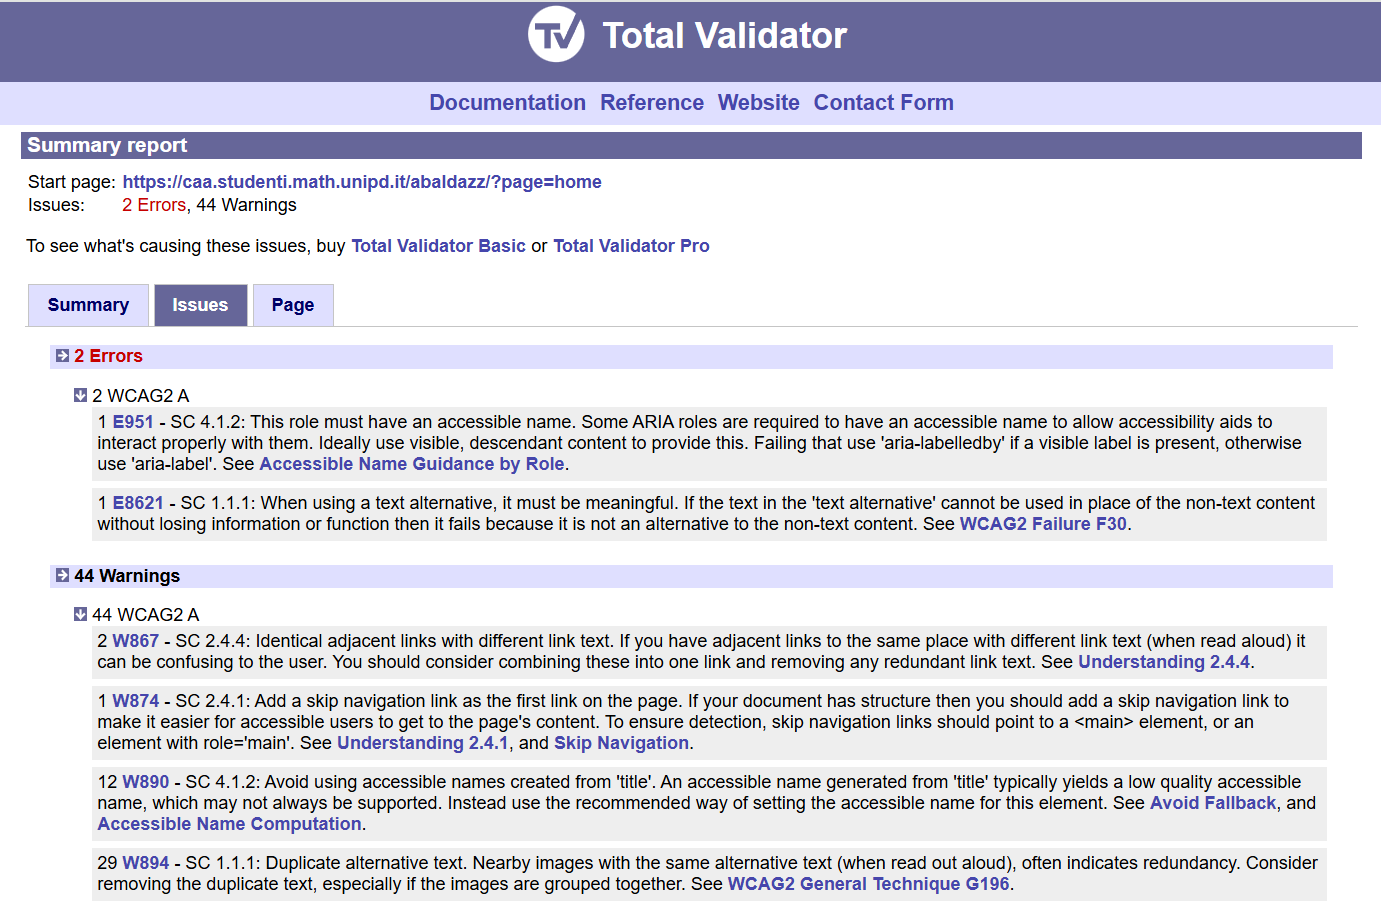
\includegraphics[width=0.8\linewidth, alt={Screenshot dell'analisi di Total Validator sul sito web E-lixirium}]{img/TV_elixirium.png}
    \caption{Analisi di Total Validator sul sito web \textit{E-lixirium}}\label{fig:TV_elixirium}
\end{figure}

\noindent L'analisi (vedi figura \ref{fig:TV_elixirium}) ha rilevato 2 errori principali e 44 warning. 
Gli errori riguardano principalmente elementi con ruoli ARIA a cui non è stato associato un nome accessibile e testi alternativi non significativi. Tra i warning, i più frequenti sono duplicazioni di testo alternativo per immagini, nomi accessibili generati da attributi \texttt{title}, link adiacenti con testi diversi e l’assenza di link di navigazione rapida. 

\subsubsection{Lighthouse}
\noindent Il report ha restituito un punteggio di 96/100 nella sezione \textit{Accessibility} (vedi figura \ref{fig:Lighthouse_elixirium}). 
Il problema segnalato riguarda il contrasto insufficiente tra colori di sfondo e primo piano, che può ridurre la leggibilità per alcuni utenti. 
\begin{figure}[H]
    \centering
    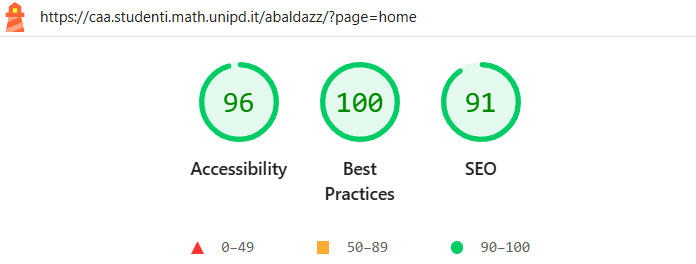
\includegraphics[width=0.6\linewidth, alt={Screenshot dell'analisi di Lighthouse sul sito web E-lixirium}]{img/Lighthouse_elixirium.png}
    \caption{Analisi di Lighthouse sul sito web \textit{E-lixirium}}\label{fig:Lighthouse_elixirium}
\end{figure}

\subsubsection{SviluppAbile}
\noindent Di seguito viene illustrato il processo di test effettuato da \textit{SviluppAbile} confrontando i risultati ottenuti dagli altri strumenti di validazione e integrando anche un controllo manuale basato sulle Web Content Accessibility Guidelines (WCAG 2.1). Lo studio è stato articolato sulle principali pagine del sito.\\

\noindent \textbf{Pagina home}\\
La pagina contiene sezioni dedicate al logo, alla navigazione e alla presentazione di categorie e prodotti. L’estensione ha rilevato alcune criticità principali: immagini dei prodotti prive di testi alternativi significativi ({\wcagref[wcag:1.1.1]{\textit{1.1.1 - Non-text Content}}}), link adiacenti con testi diversi ma comportamento simile ({\wcagref[wcag:2.4.4]{\textit{2.4.4}}}) ed elementi della navbar nascosti tramite \texttt{display:none} invece di \texttt{visibility:hidden} ({\wcagref[wcag:2.1.1]{\textit{2.1.1 - Keyboard}}}).\\
L’analisi tramite strumenti automatici ha evidenziato ulteriori problemi: assenza di skip link per saltare la navigazione ({\wcagref[wcag:2.4.1]{\textit{2.4.1 - Bypass Blocks}}}) e link duplicati o circolari nella barra di navigazione ({\wcagref[wcag:2.4.4]{\textit{2.4.4}}}). Un ulteriore problema non rilevato da \textit{SviluppAbile} riguarda il logo con link circolare verso la homepage anche quando l’utente è già nella homepage stessa ({\wcagref[wcag:2.4.4]{\textit{2.4.4 - Link Purpose (In Context)}}}).\\

\noindent \textbf{Pagina products}\\
La pagina mostra l’elenco completo dei prodotti disponibili nel negozio \textit{E-lixirium}. Come per la homepage, si riscontrano criticità di accessibilità significative: le immagini dei prodotti utilizzano come testo alternativo il nome del file ({\wcagref[wcag:1.1.1]{\textit{1.1.1}}}), le stelle di valutazione dei prodotti hanno alt duplicati o poco descrittivi ({\wcagref[wcag:1.1.1]{\textit{1.1.1}}}), e non è presente uno skip link per saltare la navigazione ({\wcagref[wcag:2.4.1]{\textit{2.4.1}}}).\\
Gli ulteriori problemi rilevati dagli strumenti automatici sono gli stessi rilevati nella homepage.\\

\noindent \textbf{Pagina about}\\
La pagina \texttt{about} presenta informazioni sull’azienda e la sua missione, con testo descrittivo e un’immagine illustrativa. Dal punto di vista dell’accessibilità, si riscontrano le stesse criticità delle pagine precedenti: l’immagine ha un testo alternativo generico (\texttt{About E-lixirium}) che non descrive il contenuto visivo in dettaglio ({\wcagref[wcag:1.1.1]{\textit{1.1.1}}}).\\
La struttura della pagina non prevede skip link per saltare la navigazione principale ({\wcagref[wcag:2.4.1]{\textit{2.4.1}}}) e non tutti i link sono chiaramente descrittivi nel contesto ({\wcagref[wcag:2.4.4]{\textit{2.4.4}}}). Inoltre, l'estensione avvisa che le informazioni contenute nella pagina sono incomplete rispetto a ciò che ci si aspetta da tale pagina (mancanza di infomrazioni di contatto per esempio).\\

\noindent \textbf{Conclusioni}\\
L’analisi complessivamente evidenzia una serie di criticità ricorrenti, in particolare relative ai testi alternativi delle immagini, alla gestione della navigazione e al contrasto visivo degli elementi interattivi. Le problematiche riscontrate potrebbero ostacolare l’accesso al sito da parte di utenti con disabilità visive o che utilizzano ausili tecnologici. Vengono anche consigliati miglioramente su alcune pagine del sito web, come l'aggiunta di informazioni per gli utenti e di testi alternativi più descrittivi.

\paragraph{F1-score} \mbox{}\\
\noindent Nella tabella \ref{tab:elixirium} vengono riportati i risultati ottenuti utilizzando l'estensione \textit{SviluppAbile}.
\begin{footnotesize}
\begin{longtable}[c]{|C{4.8cm}|C{4.8cm}|C{4.8cm}|}
\caption{Tabella riassuntiva analisi \textit{E-lixirium} tramite \textit{SviluppAbile}}
\label{tab:elixirium}\\
\hline
\textbf{Errori trovati} & \textbf{Errori non trovati} & \textbf{Falsi positivi}\\
\hline
\endfirsthead
\multicolumn{3}{c}%
{{\bfseries Tabella \thetable\ -- continua dalla pagina precedente}} \\
\hline
\textbf{Errori trovati} & \textbf{Errori non trovati} & \textbf{Falsi positivi}\\
\hline
\endhead
\hline
\multicolumn{3}{r}{{ -- continua nella pagina successiva}} \\
\endfoot
\hline
\endlastfoot
\begin{itemize}
    \item Errori di gestione della navigazione
    \item "display: none" da sostituire con "visibility: hidden"
    \item Link adiacenti identici con testi diversi
    \item Testo alternativo duplicato
\end{itemize}
 & 
\begin{itemize}
    \item Skip navigation link
    \item Link circolari nella navbar
    \item Logo con reindirizzamento nella home anche in home stesso
\end{itemize}
 & \\
\hhline{|=|=|=|} 
4 & 3 & 0 \\
\end{longtable}
\end{footnotesize}

\noindent L'F\textsubscript{1}-score calcolato è $F_{1}=0.73$, un risultato positivo che evidenzia come l’estensione abbia individuato correttamente la maggior parte degli errori presenti, pur lasciando tre problemi non rilevati. Non sono stati generati falsi positivi, il che indica un buon equilibrio tra precisione e completezza dell’analisi.


% === CORSA IDEALE ===
\subsection{Sito web: Corsa Ideale}
\noindent Di seguito vengono riportati alcuni dei test effettuati sul sito web \href{https://caa.studenti.math.unipd.it/epinarel/}{Corsa Ideale}.
\subsubsection{Total Validator}
\begin{figure}[H]
    \centering
    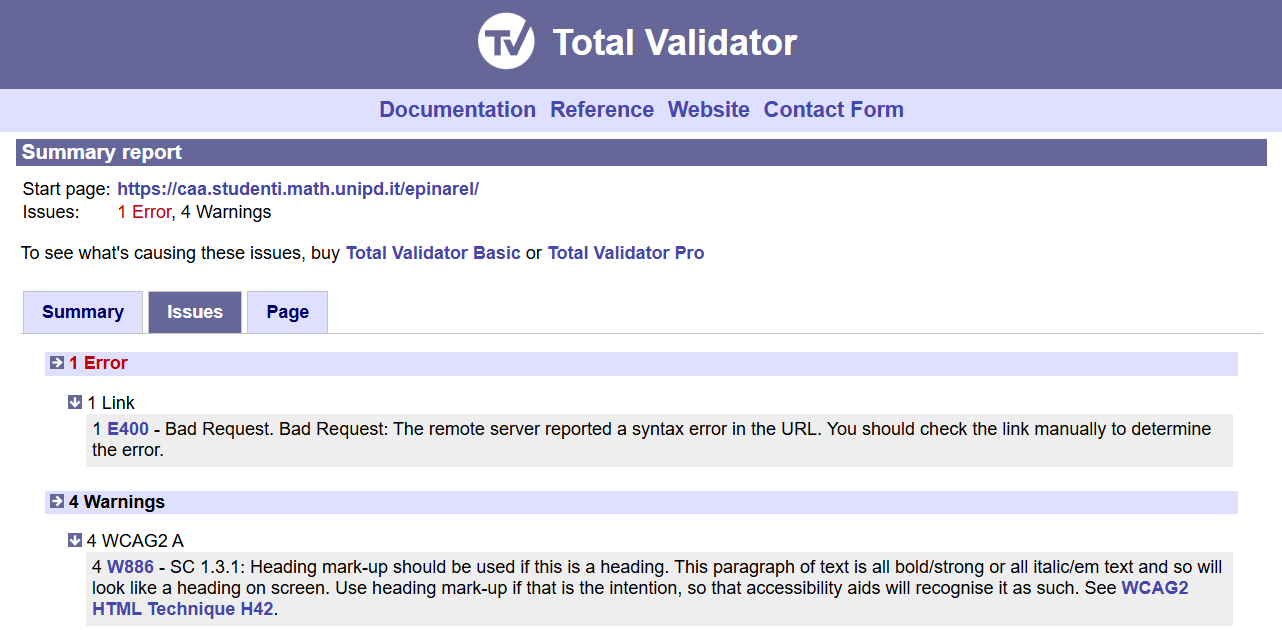
\includegraphics[width=0.8\linewidth, alt={Screenshot dell'analisi di Total Validator sul sito web Corsa Ideale}]{img/TV_corsaideale.png}
    \caption{Analisi di Total Validator sul sito web \textit{Corsa Ideale}}\label{fig:TV_corsaideale}
\end{figure}

\noindent \noindent L’analisi ha evidenziato un solo errore riguardante i link, dovuto a una richiesta non valida (\textit{Bad Request}), e quattro avvisi relativi all’uso improprio della marcatura tipografica (testi interamente in grassetto o corsivo che dovrebbero essere definiti come intestazioni). Questi warning non compromettono direttamente l’accessibilità, ma indicano buone pratiche di struttura da rispettare per garantire una corretta interpretazione da parte degli strumenti assistivi.

\subsubsection{Lighthouse}
\noindent Il report ha restituito un punteggio di 100/100 nella sezione \textit{Accessibility}, indicando che, secondo le metriche automatiche adottate, non sono stati rilevati errori o problematiche di accessibilità (vedi figura \ref{fig:Lighthouse_corsaideale}). 
Il problema segnalato riguarda il contrasto insufficiente tra colori di sfondo e primo piano, che può ridurre la leggibilità per alcuni utenti. 
\begin{figure}[H]
    \centering
    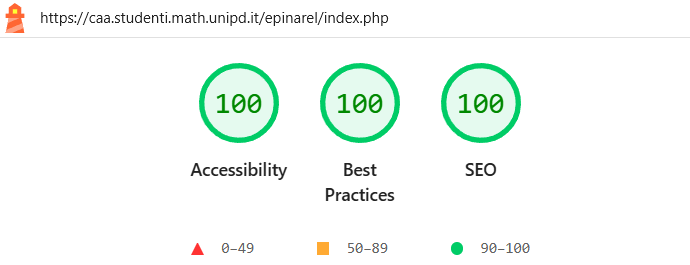
\includegraphics[width=0.6\linewidth, alt={Screenshot dell'analisi di Lighthouse sul sito web Corsa Ideale}]{img/Lighthouse_corsaideale.png}
    \caption{Analisi di Lighthouse sul sito web \textit{Corsa Ideale}}\label{fig:Lighthouse_corsaideale}
\end{figure}

\subsubsection{SviluppAbile}
\noindent Di seguito viene illustrato il processo di test effettuato da \textit{SviluppAbile} confrontando i risultati ottenuti dagli altri strumenti di validazione e integrando anche un controllo manuale basato sulle Web Content Accessibility Guidelines (WCAG 2.1). Lo studio è stato articolato sulle principali pagine del sito.\\

\noindent \textbf{Pagina home}\\
La pagina presenta il sito \texttt{CorsaIdeale}, con sezioni dedicate alla navigazione, alla presentazione delle ultime uscite, ai servizi offerti e ai ruoli dei corridori. Dal punto di vista dell’accessibilità, si riscontrano le seguenti criticità principali: immagini dei prodotti e del logo prive di testi alternativi significativi ({\wcagref[wcag:1.1.1]{\textit{1.1.1 - Non-text Content}}}), attributi \texttt{id} senza valore descrittivo o duplicati ({\wcagref[wcag:2.4.4]{\textit{2.4.4 - Link Purpose (In Context)}}}) ed etichette \texttt{label} non univoche ({\wcagref[wcag:3.3.2]{\textit{3.3.2 - Labels or Instructions}}}), .\\
La struttura della pagina prevede uno skip link per saltare la navigazione ({\wcagref[wcag:2.4.1]{\textit{2.4.1}}}), ma non tutti i link della navbar sono chiaramente descrittivi nel contesto ({\wcagref[wcag:2.4.4]{\textit{2.4.4}}}). Inoltre, non vengono utilizzati attributi ARIA aggiuntivi per migliorare la fruibilità tramite lettori di schermo, e alcune immagini decorative o informative non hanno alt appropriato ({\wcagref[wcag:1.1.1]{\textit{1.1.1}}}). Questi due ultimi errori segnalati rappresentano in realtà falsi positivi; come visto anche nei test precedenti \textit{SviluppAbile} tende a correggere erroreamente alt e ARIA.\\
Non sono stati riscontrati problemi relativi al contrasto dei colori ({\wcagref[wcag:1.4.3]{\textit{1.4.3 - Contrast (Minimum)}}}), rilevabili invece dagli altri strumenti di controllo dell'accessibilità.\\

\noindent \textbf{Pagina lista}\\ 
La pagina mostra l’elenco delle scarpe con funzionalità di ricerca, filtro e ordinamento. 
L’estensione \textit{SviluppAbile} ha rilevato alcune criticità principali: assenza di testo alternativo significativo per le immagini delle scarpe e per il logo della navbar ({\wcagref[wcag:1.1.1]{\textit{1.1.1}}}), utilizzo di \texttt{onclick} su interi blocchi cliccabili senza alternative da tastiera ({\wcagref[wcag:2.1.1]{\textit{2.1.1 - Keyboard}}}). L'estensione rileva inoltre che i nomi degli attributi sono scritti in maiuscolo anziché in minuscolo ({\wcagref[wcag:4.1.1]{\textit{4.1.1 - Parsing}}}).\\
L’analisi tramite strumenti di accessibilità ha evidenziato ulteriori problematiche: mancanza di landmark semantici coerenti come <main> e <nav> per ciascun blocco funzionale ({\wcagref[wcag:1.3.1]{\textit{1.3.1}}}) ed etichette ridondanti o generiche nei pulsanti di filtro ({\wcagref[wcag:2.4.6]{\textit{2.4.6 - Headings and Labels}}}).\\

\noindent \textbf{Pagina chi-siamo}\\
La pagina presenta informazioni sull’azienda, i valori e il team di CorsaIdeale. 
L’estensione ha rilevato alcune criticità principali: immagini senza testo alternativo significativo, compreso il logo e le foto dei membri del team ({\wcagref[wcag:1.1.1]{\textit{1.1.1}}}), uso di \texttt{onclick} sui link del menu mobile senza alternative da tastiera ({\wcagref[wcag:2.1.1]{\textit{2.1.1}}}).\\
L’analisi tramite strumenti automatici ha evidenziato ulteriori problematiche: mancanza di landmark semantici coerenti e completi per ciascun blocco di contenuto ({\wcagref[wcag:1.3.1]{\textit{1.3.1}}}), etichette generiche o mancanti per alcuni link e pulsanti ({\wcagref[wcag:2.4.6]{\textit{2.4.6}}}) e testi alternativi vuoti o poco descrittivi per le icone e immagini illustrative ({\wcagref[wcag:1.1.1]{\textit{1.1.1}}}).\\

\noindent \textbf{Pagina registrati}\\
La pagina consente agli utenti di registrarsi ed accedere alle funzionalità del sito \textit{CorsaIdeale}. 
L’estensione \textit{SviluppAbile} ha rilevato alcune criticità principali: immagini del logo e del pulsante "torna su" prive di testo alternativo significativo ({\wcagref[wcag:1.1.1]{\textit{1.1.1}}}) e campi del form con placeholder utilizzati come unica indicazione ({\wcagref[wcag:2.4.6]{\textit{2.4.6}}}). Viene inoltre segnalato l'errore di chiusura di un tag \texttt{p} con un tag \texttt{h3} ({\wcagref[wcag:1.3.1]{\textit{1.3.1 - Info and Relationships}}}).\\

\noindent \textbf{Conclusioni}\\
L’analisi complessiva delle principali pagine di \textit{CorsaIdeale} evidenzia criticità ricorrenti, in particolare relative ai testi alternativi delle immagini, alla gestione della navigazione e all’accessibilità dei form e dei link. Purtroppo l'estensione \textit{SviluppAbile} non è in grado di controllare i contrasti dei colori in maniera esaustiva e suggerisce spesso errori non presenti di heading scorretti.

\paragraph{F1-score} \mbox{}\\
\noindent Nella tabella \ref{tab:corsaideale} vengono riportati i risultati ottenuti utilizzando l'estensione \textit{SviluppAbile}.
\begin{footnotesize}
\begin{longtable}[c]{|C{4.8cm}|C{4.8cm}|C{4.8cm}|}
\caption{Tabella riassuntiva analisi \textit{Corsa Ideale} tramite \textit{SviluppAbile}}
\label{tab:corsaideale}\\
\hline
\textbf{Errori trovati} & \textbf{Errori non trovati} & \textbf{Falsi positivi}\\
\hline
\endfirsthead
\multicolumn{3}{c}%
{{\bfseries Tabella \thetable\ -- continua dalla pagina precedente}} \\
\hline
\textbf{Errori trovati} & \textbf{Errori non trovati} & \textbf{Falsi positivi}\\
\hline
\endhead
\hline
\multicolumn{3}{r}{{ -- continua nella pagina successiva}} \\
\endfoot
\hline
\endlastfoot
\begin{itemize}
    \item Alt immagini vuoti
    \item Attributi id senza valore valido 
    \item Chiusura tag p erroneamente con tag h3 
    \item Label non univoca 
    \item Nomi attributi in maiuscolo anziché in minuscolo
\end{itemize}
 & \begin{itemize}
    \item Contrasto colori
\end{itemize}
 & \begin{itemize}
    \item Tag di heading usati in maniera scorretta
\end{itemize}\\
\hhline{|=|=|=|} 
5 & 1 & 1 \\
\end{longtable}
\end{footnotesize}

\noindent L'F\textsubscript{1}-score calcolato è $F_{1}=0.83$, un risultato positivo che evidenzia come l’estensione abbia rilevato correttamente la maggior parte degli errori presenti, lasciando un solo problema non individuato e generando un solo falso positivo.


% === BOOKOVERFLOW ===
\subsection{Sito web: BookOverflow}
\noindent Di seguito vengono riportati alcuni dei test effettuati sul sito \href{https://caa.studenti.math.unipd.it/lribon/}{BookOverflow}, sito web vincitore del concorso.
\subsubsection{Total Validator}
\begin{figure}[H]
    \centering
    
\includegraphics[width=0.8\linewidth, alt={Screenshot dell'analisi di Total Validator sul sito web BookOverflow}]{img/TV_bookoverflow.png}
    \caption{Analisi di Total Validator sul sito web \textit{BookOverflow}}\label{fig:TV_bookoverflow}
\end{figure}

\noindent Come visibile in figura \ref{fig:TV_bookoverflow}, non vi sono errori di accessibilità.

\subsubsection{Lighthouse}
\noindent Il report ha restituito un punteggio di 100/100 nella sezione \textit{Accessibility}, indicando che, secondo le metriche automatiche adottate, non sono stati rilevati errori o problematiche di accessibilità (vedi figura \ref{fig:Lighthouse_bookoverflow}).
\begin{figure}[H]
    \centering
    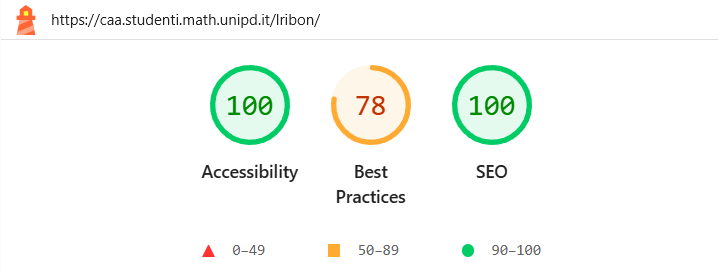
\includegraphics[width=0.6\linewidth, alt={Screenshot dell'analisi di Lighthouse sul sito web BookOverflow}]{img/Lighthouse_bookoverflow.png}
    \caption{Analisi di Lighthouse sul sito web \textit{BookOverflow}}\label{fig:Lighthouse_bookoverflow}
\end{figure}

\subsubsection{SviluppAbile}
\noindent Di seguito viene illustrato il processo di test effettuato da \textit{SviluppAbile} confrontando i risultati ottenuti dagli altri strumenti di validazione e integrando anche un controllo manuale basato sulle Web Content Accessibility Guidelines (WCAG 2.1). Lo studio è stato articolato sulle principali pagine del sito.\\

\noindent \textbf{Pagina home}\\
La pagina introduce la piattaforma e mostra i libri più scambiati. 
L’estensione \textit{SviluppAbile} segnala un uso inappropriato del tabindex sugli elementi interattivi ({\wcagref[wcag:2.1.1]{\textit{2.1.1}}}).\\
L’analisi ha confermato invece che tutti gli elementi interattivi sono correttamente accessibili, dall'analisi manuale invece si può notare che sembra non esservi un contrasto sufficiente tra link visitati e non visitati ({\wcagref[wcag:1.4.3]{\textit{1.4.3}}}).\\

\noindent \textbf{Pagina esplora}\\
La pagina consente agli utenti di scoprire nuovi libri, visualizzare i titoli più popolari e accedere a contenuti personalizzati dopo il login. 
L’estensione \textit{SviluppAbile} ha segnalato falsi positivi per uso inappropriato del tabindex sugli elementi interattivi ({\wcagref[wcag:2.1.1]{\textit{2.1.1}}}).\\
L’analisi manuale ha confermato che tutti i link e i pulsanti sono etichettati in modo chiaro e tutte le immagini decorative o informative dispongono di testo alternativo appropriato ({\wcagref[wcag:1.1.1]{\textit{1.1.1}}}, {\wcagref[wcag:1.3.1]{\textit{1.3.1}}}, {\wcagref[wcag:2.4.6]{\textit{2.4.6}}}). Inoltre, i contenuti personalizzati richiedono il login, ma i messaggi indicano chiaramente come accedere, senza compromettere l’accessibilità.\\

\noindent \textbf{Pagina come-funziona}\\
La pagina illustra il funzionamento della piattaforma \textit{BookOverflow}, spiegando agli utenti i vantaggi dello scambio libri e guidandoli passo passo attraverso la creazione della libreria, la selezione dei desideri e le modalità di spedizione. 
L’estensione \textit{SviluppAbile} non segnala alcun tipo di errore.\\

\noindent \textbf{Conclusioni}\\
In sintesi, la pagina risulta pienamente accessibile; le criticità segnalate da \textit{SviluppAbile} costituiscono falsi positivi dovuti alle ristrette capacità di analisi dell'IA alla base dell'estensione.\\


\paragraph{F1-score} \mbox{}\\
\noindent Nella tabella \ref{tab:bookoverflow} vengono riportati i risultati ottenuti utilizzando l'estensione \textit{SviluppAbile}.
\begin{footnotesize}
\begin{longtable}[c]{|C{4.8cm}|C{4.8cm}|C{4.8cm}|}
\caption{Tabella riassuntiva analisi \textit{BookOverflow} tramite \textit{SviluppAbile}}
\label{tab:bookoverflow}\\
\hline
\textbf{Errori trovati} & \textbf{Errori non trovati} & \textbf{Falsi positivi}\\
\hline
\endfirsthead
\multicolumn{3}{c}%
{{\bfseries Tabella \thetable\ -- continua dalla pagina precedente}} \\
\hline
\textbf{Errori trovati} & \textbf{Errori non trovati} & \textbf{Falsi positivi}\\
\hline
\endhead
\hline
\multicolumn{3}{r}{{ -- continua nella pagina successiva}} \\
\endfoot
\hline
\endlastfoot
 & 
\begin{itemize}
    \item Contrasto insufficiente link visitati/non
\end{itemize}
 & \begin{itemize}
    \item Tabindex non adeguato
\end{itemize}\\
\hhline{|=|=|=|} 
0 & 1 & 1 \\
\end{longtable}
\end{footnotesize}

\noindent L'F\textsubscript{1}-score calcolato è $F_{1}=0$, valore che indica prestazioni non soddisfacenti in questo caso specifico. 
Ciò evidenzia la necessità di ulteriori miglioramenti nell’identificazione degli errori, soprattutto per quanto riguarda i falsi positivi.

% === LUZZAUTO ===
\subsection{Sito web: LuzzAuto}
\noindent Di seguito vengono riportati alcuni dei test effettuati sul sito web \href{https://caa.studenti.math.unipd.it/eartusi/index.php}{LuzzAuto}.
\subsubsection{Total Validator}
\begin{figure}[H]
    \centering
    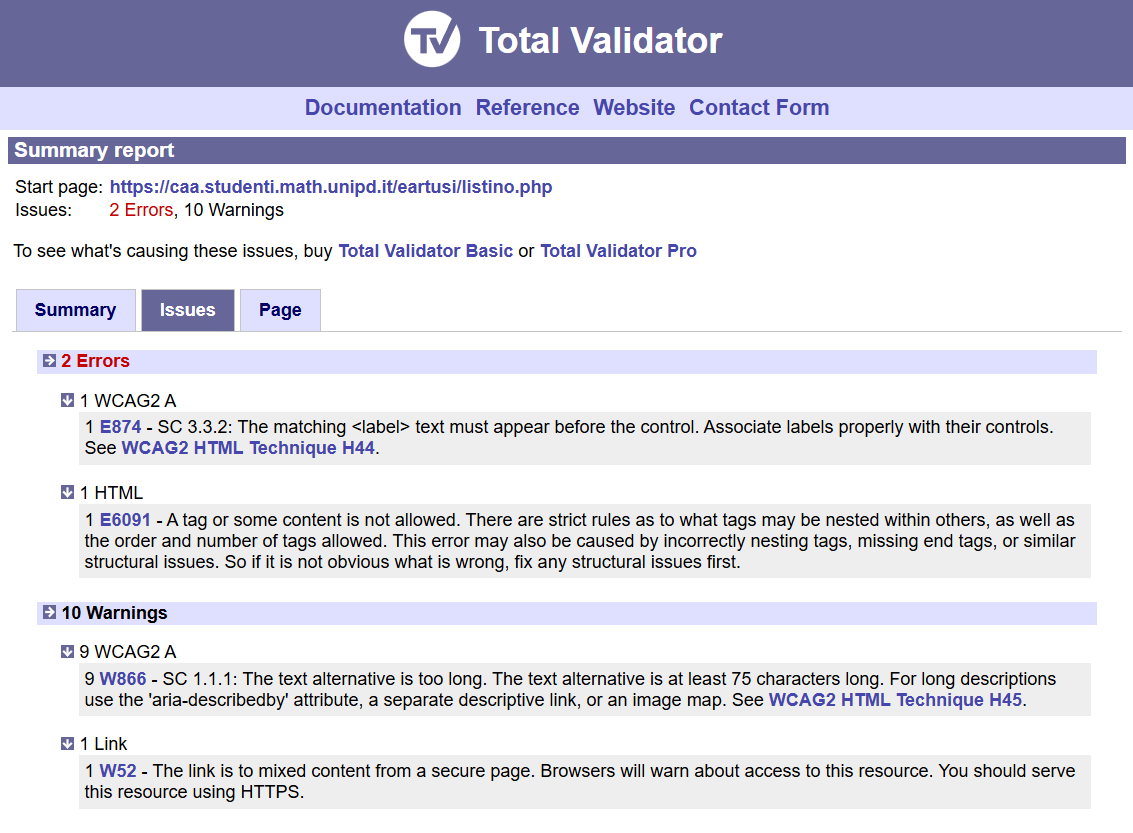
\includegraphics[width=0.8\linewidth, alt={Screenshot dell'analisi di Total Validator sul sito web LuzzAuto}]{img/TV_luzzauto.png}
    \caption{Analisi di Total Validator sul sito web \textit{LuzzAuto}}\label{fig:TV_luzzauto}
\end{figure}

\noindent Nella pagina \texttt{home.php} non sono presenti errori di accessibilità, ma solamente un "Warning" riguardante testi alternativi (\texttt{alt}) troppo lunghi. 
Nella pagina \texttt{listino.php} (come visibile in figura \ref{fig:TV_luzzauto}), sono segnalati due errori principali: 
uno relativo all'associazione corretta delle etichette ai rispettivi controlli e uno di struttura HTML, dovuto all'uso di tag non consentiti o a un errato annidamento degli stessi. 

\subsubsection{Lighthouse}
\noindent Il report ha restituito un punteggio di 100/100 nella sezione \textit{Accessibility}, indicando che, secondo le metriche automatiche adottate, non sono stati rilevati errori o problematiche di accessibilità (vedi figura \ref{fig:Lighthouse_luzzauto}).
\begin{figure}[H]
    \centering
    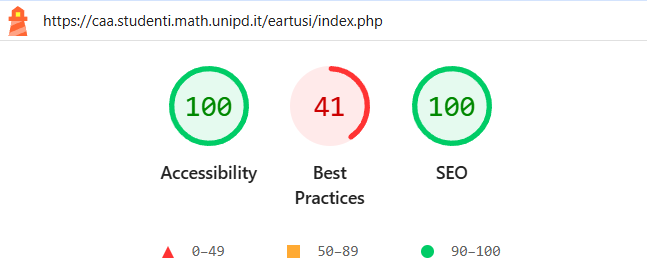
\includegraphics[width=0.6\linewidth, alt={Screenshot dell'analisi di Lighthouse sul sito web LuzzAuto}]{img/Lighthouse_luzzauto.png}
    \caption{Analisi di Lighthouse sul sito web \textit{LuzzAuto}}\label{fig:Lighthouse_luzzauto}
\end{figure}

\subsubsection{SviluppAbile}
\noindent Di seguito viene illustrato il processo di test effettuato da \textit{SviluppAbile} confrontando i risultati ottenuti dagli altri strumenti di validazione e integrando anche un controllo manuale basato sulle Web Content Accessibility Guidelines (WCAG 2.1). Lo studio è stato articolato sulle principali pagine del sito.\\

\noindent \textbf{Pagina home}\\
L’analisi della pagina tramite l’estensione \textit{SviluppAbile} non ha rilevato errori di accessibilità. L’unico avviso segnalato riguarda testi alternativi (\texttt{alt}) troppo lunghi per alcune immagini, ma queste descrizioni dettagliate non compromettono la fruibilità dei contenuti per utenti con disabilità visive ({\wcagref[wcag:1.1.1]{\textit{1.1.1 - Non-text Content}}}). \\

\noindent \textbf{Pagina about}\\
L’analisi della pagina non ha evidenziato errori di accessibilità e sono stati correttamente individuati gli elementi interattivi come link e pulsanti, che risultano etichettati e navigabili tramite tastiera ({\wcagref[wcag:2.1.1]{\textit{2.1.1}}}), garantendo la conformità ai requisiti WCAG relativi all’accessibilità da tastiera e alla comprensibilità dei contenuti testuali.  
La pagina presenta una struttura semantica chiara ({\wcagref[wcag:1.3.1]{\textit{1.3.1 - Info and Relationships}}}), immagini corredate da testi alternativi descrittivi ({\wcagref[wcag:1.1.1]{\textit{1.1.1}}}) e informazioni accessibili sulle sezioni del sito.\\

\noindent \textbf{Pagina test\_drive}\\
L’analisi della pagina non ha rilevato errori di accessibilità.\\

\noindent \textbf{Conclusioni}\\
L’analisi complessiva delle pagine principali tramite \textit{SviluppAbile} mostra che l’estensione è efficace nell’individuare problemi come testi alternativi troppo lunghi e garantire la navigabilità da tastiera degli elementi interattivi. Tuttavia, alcune criticità relative alla struttura HTML, all’uso corretto dei tag semantici e alla compatibilità con lettori di schermo non vengono completamente rilevate.  
È pertanto consigliabile integrare l’uso di \textit{SviluppAbile} con controlli manuali e verifiche basate sulle WCAG 2.1 ({\wcagref[wcag:1.1.1]{\textit{1.1.1}}}, {\wcagref[wcag:1.3.1]{\textit{1.3.1}}}, {\wcagref[wcag:2.1.1]{\textit{2.1.1}}}, {\wcagref[wcag:4.1.1]{\textit{4.1.1}}}) per ottenere una valutazione completa dell’accessibilità del sito.


\paragraph{F1-score} \mbox{}\\
\noindent Nella tabella \ref{tab:luzzauto} vengono riportati i risultati ottenuti utilizzando l'estensione \textit{SviluppAbile}.
\begin{footnotesize}
\begin{longtable}[c]{|C{4.8cm}|C{4.8cm}|C{4.8cm}|}
\caption{Tabella riassuntiva analisi \textit{LuzzAuto} tramite \textit{SviluppAbile}}
\label{tab:luzzauto}\\
\hline
\textbf{Errori trovati} & \textbf{Errori non trovati} & \textbf{Falsi positivi}\\
\hline
\endfirsthead
\multicolumn{3}{c}%
{{\bfseries Tabella \thetable\ -- continua dalla pagina precedente}} \\
\hline
\textbf{Errori trovati} & \textbf{Errori non trovati} & \textbf{Falsi positivi}\\
\hline
\endhead
\hline
\multicolumn{3}{r}{{ -- continua nella pagina successiva}} \\
\endfoot
\hline
\endlastfoot
\begin{itemize}
    \item Le etichette dei controlli non sono state associate correttamente ai rispettivi elementi.
\end{itemize} & 
\begin{itemize}
    \item Tag o contenuto non consentito. 
\end{itemize}
 & \\
\hhline{|=|=|=|} 
1 & 1 & 0 \\
\end{longtable}
\end{footnotesize}

\noindent L'F\textsubscript{1}-score calcolato è $F_{1} \approx 0.67$, un valore intermedio che evidenzia un discreto equilibrio tra errori rilevati e mancati. 
Pur non trattandosi di un risultato ottimale, esso mostra la capacità dell’estensione di individuare correttamente una parte significativa dei problemi, lasciando spazio a ulteriori miglioramenti.

\section{Test ``Modalità guidata''}
\noindent Per effettuare i test utili a dimostrare l'efficacia di \textit{SviluppAbile}, ho creato una semplice pagina \acrshort{html} (vedi figura \ref{fig:pagina_test}).
\begin{figure}[H]
    \centering
    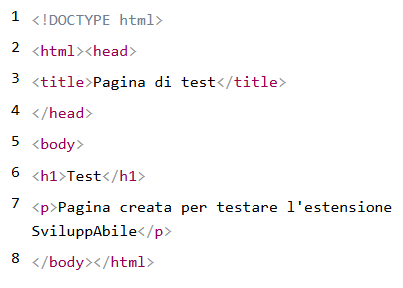
\includegraphics[width=0.5\linewidth, alt={Pagina \acrshort{html} base per effettuare i test della modalità guidata}]{img/test_MG.png}
    \caption{Pagina HTML base per effettuare i test della modalità guidata}\label{fig:pagina_test}
\end{figure}

\subsubsection*{\texttt{Come si crea un <head> che contenga tutti gli elementi utili per una pagina accessibile?}}
\begin{adjustwidth}{1cm}{1cm}
\noindent {\footnotesize Per creare un head accessibile, assicurati di includere i seguenti elementi:\\
1.  **Metatag Titolo (title)**: Utilizzato dal browser come titolo della finestra della pagina.\\
2.  **Metatag Descrizione (description)**: Descrive il contenuto della pagina e appare nella barra degli strumenti del browser e nei risultati dei motori di ricerca.\\
3.  **Metatag Chiave (keywords)**: Non più importante come in passato, ma puoi utilizzarla se necessario per le ricerche.\\
\\Inoltre, assicurati di utilizzare un markup semantico corretto per le sezioni della pagina. Ad esempio, puoi utilizzare `<header>`, `<nav>`, `<main>`, `<section>`, `<article>`, `footer>` in luogo di semplici div.\\
Infine, assicurati di aggiungere un elemento `alt` a tutte le immagini con una descrizione del contenuto dell'immagine.\\
\\CODICE SUGGERITO:\\
\texttt{1 <head>\\
2 <title>Pagina di test</title>\\
3 <meta charset="UTF-8">\\
4 <meta name="viewport" content="width=device-width, initial-scale=1.0">\\
5 <meta name="description" content="Pagina creata per testare l'estensione SviluppAbile">\\
6 <meta name="keywords" content="test,sviluppo accessibile">\\
7 </head>\\}}
\end{adjustwidth}


\subsubsection*{\texttt{Come posso ora creare dei paragrafi che rispettino le linee guida BEM?}}
\begin{adjustwidth}{1cm}{1cm}
\noindent {\footnotesize Per creare paragrafi in base alle linee guida BEM, puoi utilizzare la sintassi seguente:\\
1. Definisci un classico `.block\_\_element` per il contenuto del paragrafo: `class="block\_\_element"`\\
2. Utilizza `.block\_\_element--modificatore` per aggiungere modificatori: `class="block\_\_element --modificatore"`\\
In questo modo, i paragrafi saranno distinti e facili da identificare tramite la tecnica BEM.\\
\\Nota: Assicurati di sostituire `--modificatore` con il nome del modificatore effettivo nel tuo progetto.\\
\\CODICE SUGGERITO:\\
\texttt{1 <h1 class="block\_\_title">Titolo</h1>\\
2 <p class="block\_\_text --grande">Testo di esempio con un modificatore per il colore.</p>\\
3 <p class="block\_\_text --rosso">Testo di esempio con altro contenuto.</p>}\\
}
\end{adjustwidth}


\subsubsection*{\texttt{Come posso inserire immagini accessibili?}}
\begin{adjustwidth}{1cm}{1cm}
\noindent {\footnotesize Inserire immagini accessibili significa garantire che le informazioni contenute nelle immagini siano anche disponibili ai utenti con disabilità visiva. Ciò può essere fatto utilizzando l'attributo `alt` all'interno dell'elemento `<img>`.\\
In questo esempio, l'attributo `alt` contiene una descrizione breve e concisa della foto. Se il browser non è in grado di visualizzare l'immagine (ad esempio, se si utilizza un lettore schermo), la descrizione contenuta nell'attributo `alt` verrà visualizzata al posto dell'immagine.\\
Inoltre, per immagini decorative o grafici che non contengono informazioni importanti, è consigliabile utilizzare l'attributo `alt=""`, in modo da eliminare il testo alternativo dalla navigazione.\\
\\CODICE SUGGERITO:\\
\texttt{1 <img src="immagine.jpg" alt="Descrizione della foto">}
}
\end{adjustwidth}

\subsubsection*{\texttt{Come si crea una table rispettando le linee guida WCAG?}}
\begin{adjustwidth}{1cm}{1cm}
\noindent {\footnotesize Per creare una tabella accessibile secondo le linee guida WCAG, è importante fornire un'esperienza utente inclusiva e facilitare l'accessibilità a tutte le persone, in particolare alle persone con disabilità visive che utilizzano strumenti di lettura ad alta voce o tastiera. Ecco alcuni passaggi per creare una tabella accessibile:\\
1.  **Istruzioni per l'utilizzo della tabella**: fornire un'introduzione sulle informazioni presentate nella tabella e quali sono le colonne principali, aiutando gli utenti che utilizzano strumenti di lettura ad alta voce.\\
2.  **Tabella semantica con role="presentation" impostato su false**: questo ti permetterà a un assistente di lettura di comprendere il contenuto della tabella e fornirlo correttamente all'utente.\\
\\Nota che ogni elemento della tabella (celle, intestazioni) deve avere un id o un attributo aria-*, per fornire una descrizione dell'elemento e aiutare gli utenti con disabilità visive a comprendere il contenuto.\\
\\CODICE SUGGERITO:\\
\texttt{1 <table>\\
2 <caption>Esempio di tabella accessibile</caption>\\
3 <thead>\\
4 <tr role="row">\\
5 <th scope="col" id="nome">Nome</th>\\
6 <th scope="col" id="età">Età</th>\\
7 </tr>\\
8 </thead>\\
9 <tbody>\\
10 <tr role="row">\\
11 <td headers="nome">Mario Rossi</td>\\
12 <td headers="età">32 anni</td>\\
13 </tr>\\
14 <tr role="row">\\
15 <td headers="nome">Giovanni Bianchi</td>\\
16 <td headers="età">35 anni</td>\\
17 </tr>\\
18 </tbody>\\
19 </table>}
}
\end{adjustwidth}


\subsubsection*{\texttt{Come posso utilizzare gli attributi ARIA per migliorare l'accessibilità degli elementi interattivi?}}
\begin{adjustwidth}{1cm}{1cm}
\noindent {\footnotesize Gli attributi ARIA (Accessible Rich Internet Applications) sono stati sviluppati per rendere le applicazioni web accessibili a tutti, nonostante eventuali disabilità. Sono utilizzati per aggiungere funzionalità di navigazione e controllo agli elementi interattivi come i bottoni e gli elementi dropdown.\\
Per migliorare l'accessibilità degli elementi interattivi tramite ARIA, ti suggerisco di utilizzare le seguenti strategie:\\
1.  Utilizza il role di un elemento (ad esempio `button`, `menuitem`) per specificarne la funzione.\\
2.  Aggiungi gli attributi aria-label e aria-describedby per fornire una descrizione dell'elemento interattivo.\\
3.  Utilizza l'attributo aria-haspopup per indicare se un elemento è un menu o una lista.\\
\\In questo modo, l'elemento interattivo sarà più facile da navigare e controllare tramite strumenti assistivi come screen reader e mouse navigator.\\
Per ulteriori informazioni sugli attributi ARIA, ti consiglio di consultare la documentazione ufficiale dell'W3C.\\
\\CODICE SUGGERITO:\\
\texttt{1 <!DOCTYPE html>\\
2 <html><head>\\
3 <title>Pagina di test</title>\\
4 </head>\\
5 <body>\\
6 <!-- Utilizzo del role e degli attributi ARIA per il bottone -->\\
7 <button role="button" aria-label="Clicca per eseguire l'azione"> Esegui azione </button>\\
8 <!-- Utilizzo del role e degli attributi ARIA per il menu -->\\
9 <ul role="menu">\\
10 <li role="presentation">\\
11 <a href="\#" aria-label="Opzione 1" aria-haspopup="true">Opzione 1</a>\\
12 <ul role="sottomenu">\\
13 <li role="presentation"><a href="\#" aria-label="Sottopagina 1.1">Sottopagina 1.1</a></li>\\
14 <li role="presentation"><a href="\#" aria-label="Sottopagina 1.2">Sottopagina 1.2</a></li>\\
15 </ul></li></ul>\\
16 </body></html>}
}
\end{adjustwidth}

\section{Lista WCAG citate}
\begin{itemize}
    \item \label{wcag:1.1.1} \href{https://www.w3.org/TR/WCAG21/#non-text-content}{1.1.1 - Non-text Content}
    \item \label{wcag:1.3.1} \href{https://www.w3.org/TR/WCAG21/#info-and-relationships}{1.3.1 - Info and Relationships}
    \item \label{wcag:1.4.3} \href{https://www.w3.org/TR/WCAG21/#contrast-minimum}{1.4.3 - Contrast (Minimum)}
    \item \label{wcag:1.4.4} \href{https://www.w3.org/TR/WCAG21/#resize-text}{1.4.4 - Resize Text}
    \item \label{wcag:2.1.1} \href{https://www.w3.org/TR/WCAG21/#keyboard}{2.1.1 - Keyboard}
    \item \label{wcag:2.4.1} \href{https://www.w3.org/TR/WCAG21/#bypass-blocks}{2.4.1 - Bypass Blocks}
    \item \label{wcag:2.4.2} \href{https://www.w3.org/TR/WCAG21/#page-titled}{2.4.2 - Page Titled}
    \item \label{wcag:2.4.4} \href{https://www.w3.org/TR/WCAG21/#link-purpose-in-context}{2.4.4 - Link Purpose (In Context)}
    \item \label{wcag:2.4.6} \href{https://www.w3.org/TR/WCAG21/#headings-and-labels}{2.4.6 - Headings and Labels}
    \item \label{wcag:2.4.7} \href{https://www.w3.org/TR/WCAG21/#focus-visible}{2.4.7 - Focus Visible}
    \item \label{wcag:2.4.8} \href{https://www.w3.org/TR/WCAG21/#location}{2.4.8 - Location}
    \item \label{wcag:2.4.9} \href{https://www.w3.org/TR/WCAG21/#link-purpose-link-only}{2.4.9 - Link Purpose (Link Only)}
    \item \label{wcag:3.3.1} \href{https://www.w3.org/TR/WCAG21/#error-identification}{3.3.1 - Error Identification}
    \item \label{wcag:3.3.2} \href{https://www.w3.org/TR/WCAG21/#labels-or-instructions}{3.3.2 - Labels or Instructions}
    \item \label{wcag:4.1.1} \href{https://www.w3.org/TR/WCAG21/#parsing}{4.1.1 - Parsing}
    \item \label{wcag:4.1.2} \href{https://www.w3.org/TR/WCAG21/#name-role-value}{4.1.2 - Name, Role, Value}
\end{itemize}




    \chapter{Conclusioni}
\label{chap:conclusioni}
\noindent Al termine dello stage, si può affermare che l’obiettivo principale del progetto è stato in parte raggiunto. È stata infatti realizzata un’estensione web, denominata \textit{SviluppAbile}, capace di analizzare le pagine web e assistere gli sviluppatori nell’individuazione e correzione degli errori di accessibilità. L’attività ha richiesto più fasi, tra cui la progettazione dell’architettura dell’estensione, l’implementazione delle diverse funzionalità ed una consistente fase di testing finale. \\Particolare attenzione è stata posta all’integrazione del \glslink{chatbotg}{chatbot}, concepito per fornire spiegazioni chiare e in linguaggio naturale, così da rendere i contenuti accessibili anche a chi non ha conoscenze avanzate delle linee guida \acrshort{wcag} per l'accessiilità web.

\section{Raggiungimento degli obiettivi}
\noindent Il progetto SviluppAbile ha raggiunto pienamente l’obiettivo primario di realizzare uno strumento interattivo per il supporto allo sviluppo accessibile. Sono state implementate le funzionalità principali: la visualizzazione del codice sorgente delle pagine web e la possibilità di interagire con un \glslink{chatbotg}{chatbot} integrato per analizzare la pagina web, ricevere chiarimenti e suggerimenti personalizzati.\\
Un ulteriore traguardo è stato il completamento della modalità guidata, che affianca all’analisi automatica un ambiente di sviluppo interattivo, composto da tre pannelli, in cui l’utente può sperimentare correzioni assistite del codice e scaricare direttamente i blocchi proposti in formato \acrshort{html}. Questa funzionalità ha permesso di unire l’aspetto correttivo con quello formativo, rendendo lo strumento utile sia come validatore che come supporto didattico.\\
L’architettura basata esclusivamente su tecnologie web standard, conforme a Manifest V3, ha garantito la compatibilità con i \glslink{browserg}{browser} moderni e la facilità di distribuzione dell’estensione. 
In sintesi, il sistema ha dimostrato di soddisfare gli obiettivi stabiliti: fornire uno strumento intuitivo, accessibile e formativo, capace di supportare in tempo reale lo sviluppatore nella produzione di pagine web più accessibili.\\
Per quanto riguarda invece la qualità e la completa correttezza delle risposte e del codice generato, è emerso che l’\acrshort{ia} talvolta segnala errori inesistenti o, al contrario, non rileva alcune criticità reali. Inoltre il codice proposto non sempre risulta pienamente conforme alle best-practice in materia di accessibilità. Pertanto, il miglioramento non riguarda l’estensione in sé, bensì la scelta del modello di \glslink{iag}{intelligenza artificiale} e il suo continuo affinamento.\\
In particolare, si è reso necessario identificare la versione di Ollama più congrua per le esigenze del progetto: inizialmente erano stati avviati test utilizzando sia il PC personale (versione Mistral) sia quello dell’università (versione LLaMA 3.1:8B). Successivamente è stata valutata la versione 3.2:3B, che mostrava performance migliori, ma le risposte tendevano a contenere un maggior numero di errori di formulazione e grammaticali, oltre a imprecisioni nel contenuto; per questi motivi, si è scelto di adottare per tutti i test riportati in questa tesi la versione 3.1:8b, che garantisce un equilibrio più stabile tra accuratezza e affidabilità.

\subsection{Misurazione quantitativa dei requisiti soddisfatti}
\noindent Il confronto con i requisiti inizialmente definiti (vedi paragrafo \ref{sec:req}) evidenzia quanto segue:
\begin{itemize}
    \item Requisiti obbligatori: 6/6 implementati (100\%)
    \item Requisiti desiderabili: 4/4 soddisfatti (100\%)
    \item Requisiti facoltativi: 1/3 rispettati (33\%)
\end{itemize}
Quindi il tasso di completamento complessivo è di 11/13 requisiti (84\%).

\section{Sviluppi futuri}
\noindent L’estensione web \textit{SviluppAbile} costituisce una base su cui innestare ulteriori miglioramenti: grazie alla struttura modulare, sarà possibile introdurre nuove funzionalità senza compromettere la stabilità del sistema.\\
Un primo ambito di sviluppo riguarda l’integrazione di modelli di \glslink{iag}{intelligenza artificiale} più avanzati (come \glslink{ChatGPTg}{ChatGPT} o sistemi analoghi), in grado di fornire risposte più precise, complete e soprattutto più rapide. Questo permetterebbe di aumentare l’affidabilità del \glslink{chatbotg}{chatbot} e di garantire un supporto sempre più accurato agli sviluppatori.\\
Dal punto di vista dell’interfaccia utente, potrebbe essere introdotta una scansione automatica iniziale del \acrshort{dom}, che mostri fin da subito eventuali errori in un pannello dedicato, prendendo spunto da strumenti consolidati come \textit{WAVE}.\\
\\
Un’evoluzione significativa riguarda inoltre l’integrazione di tecniche di \textit{Computer Vision}, che consentirebbero di estendere l’analisi anche agli aspetti visivi della pagina, come il contrasto cromatico, la leggibilità dei testi e le proporzioni degli elementi grafici.\\
Altri sviluppi possibili includono il collegamento con validatori esterni (come TV, WAVE e Lighthouse), l’introduzione di un versionamento dei suggerimenti generati per facilitare il confronto tra diverse soluzioni e l’ottimizzazione delle prestazioni tramite caching o caricamento progressivo del \acrshort{dom}.
In prospettiva, \textit{SviluppAbile} potrebbe evolvere in un vero e proprio laboratorio per l’accessibilità, capace di coniugare analisi automatica, supporto interattivo e verifica visiva, offrendo agli sviluppatori uno strumento ancora più completo e formativo.

\section{Consuntivo finale}
\noindent Lo sviluppo dell’estensione \textit{SviluppAbile} ha richiesto un totale di 300 ore, in linea con il monte ore preventivato. Il tempo è stato principalmente suddiviso tra lo studio del linguaggio JavaScript e l’apprendimento dello sviluppo di estensioni per \glslink{browserg}{browser}, l’integrazione dell'\glslink{iag}{intelligenza artificiale} per l’analisi del \acrshort{dom}, il ripasso delle best-practice per l'accessibilità web e le attività finali di test per verificare il corretto funzionamento e l’affidabilità dell’estensione. 

\section{Competenze acquisite}
\noindent Il progetto di stage ha rappresentato un’importante occasione di crescita tecnica e professionale, permettendo di acquisire competenze trasversali fondamentali. Dal punto di vista dello sviluppo web, l’esperienza ha consolidato la mia conoscenza di \acrshort{html}, sia nella struttura delle pagine che nella gestione degli elementi interattivi, e delle tecniche per produrre codice accessibile e semanticamente corretto. L’uso di strumenti di validazione del codice, come Total Validator, ha permesso di comprendere a fondo le problematiche legate all’accessibilità e di applicare concretamente le linee guida \acrshort{wcag} durante lo sviluppo.\\
Particolare attenzione è stata posta all’integrazione di funzionalità complesse in un ambiente modulare e compatibile con Manifest V3, comprendendo lo sviluppo di pannelli interattivi, la comunicazione tra \glslink{scriptg}{script} di background e content \glslink{scriptg}{script} e l’uso iniziale delle \acrshort{api} di Chrome. L’implementazione del \glslink{chatbotg}{chatbot} ha richiesto la selezione di un’\acrshort{ia} utilizzabile, la cui scelta è ricaduta su Ollama, nonché la generazione dinamica di domande suggerite, il filtraggio delle risposte prodotte e la sincronizzazione con il codice visualizzato nei pannelli.\\
Il progetto ha avuto un carattere sperimentale, quindi non tutte le funzionalità da sviluppare erano definite fin dall’inizio; di conseguenza, non tutte le soluzioni ipotizzate sono state realizzabili, soprattutto a causa della complessità tecnica e dei vincoli di tempo. Questa esperienza ha comunque permesso di sviluppare capacità di problem solving, adattamento e gestione autonoma delle priorità, affrontando le difficoltà tipiche della sperimentazione.\\
Infine, il progetto ha permesso di sviluppare un approccio critico all’accessibilità digitale, comprendendo a fondo le linee guida \acrshort{wcag} e le strategie per guidare gli sviluppatori nel miglioramento della qualità dei propri siti. 
\\In sintesi, l’esperienza ha combinato conoscenze teoriche e pratiche, fornendo strumenti concreti per la realizzazione di applicazioni web interattive, performanti e inclusive.

\section{Valutazione personale}
\noindent Lo svolgimento di questo progetto di stage ha rappresentato la mia prima vera esperienza di ricerca, un’occasione preziosa che mi ha permesso di andare oltre la semplice applicazione delle conoscenze acquisite durante il percorso universitario. Da un lato, ho potuto consolidare competenze tecniche già note e sperimentarne di nuove, dall’altro ho avuto l’opportunità di affrontare problemi a me sconosciuti con un approccio critico e metodologico, tipico delle attività di ricerca. Particolarmente stimolante è stata la possibilità di coniugare aspetti teorici, come i principi di accessibilità e le normative \acrshort{wcag}, con aspetti pratici legati alla realizzazione di uno strumento effettivamente utile agli sviluppatori. Ho trovato gratificante anche la libertà progettuale concessa, che mi ha spinto a sperimentare soluzioni non sempre funzionanti e a trasformare le difficoltà incontrate in momenti di crescita personale e professionale. \\
In conclusione, considero questa esperienza di stage un passaggio fondamentale del mio percorso formativo, tanto da rivalutare la possibilità di proseguire con una laurea magistrale (in \textit{Intelligenza Artificiale} oppure in \textit{Programming Languages, Systems and Algorithms}), anche se a tempo parziale.
    
    \backmatter
    \pagenumbering{roman}
    \printglossary[type=\acronymtype, title=Acronimi e abbreviazioni, toctitle=Acronimi e abbreviazioni]
    \printglossary[type=main, title=Glossario, toctitle=Glossario]
    
    \cleardoublepage
\chapter{Bibliografia}

\nocite{*}

% Print book bibliography
% \printbibliography[heading=subbibliography,title={Riferimenti bibliografici},type=book]

% Print site bibliography
\printbibliography[heading=subbibliography,title={Siti web consultati},type=online]
\end{document}